\documentclass[12pt,a4paper]{article}
\usepackage{float}
 \usepackage{natbib}    % For BibTeX
 \usepackage{graphicx}
\usepackage{bm}
\usepackage{amsfonts}% To import .pdf files
\usepackage{hyperref}
\usepackage{amsmath}
\usepackage{booktabs}
 \oddsidemargin  -10mm
 \evensidemargin -10mm
 \headheight 0mm
 \headsep -3mm
\textheight 250mm
\textwidth 180mm
\topmargin -4mm
\topskip -10mm
\usepackage{amsmath} % Include the amsmath package
%\textwidth=450pt
%\hoffset=-2cm
\usepackage{graphicx}
\usepackage{subcaption}
\usepackage{float}
\newcommand{\RR}{{\textsf{R}}}
\begin{document}

\begin{Large}
\begin{center}
\textbf{``Fast Spectral Density Estimation for \\Multivariate Time Series''} \\
\textbf{by Jianan Liu} \\
\textbf{for a PhD in Statistics}
\end{center}
\end{Large}


\hfill{Student ID: 786158628}

\hfill{Email: jliu812@aucklanduni.ac.nz}

\hfill{Department of [Statistics]}

Supervisor: Professor Renate Meyer (Main Supervisor) Dr Kate Lee (Joint Main Supervisor)

\begin{center}
Date of enrolment: 1/10/2022  
Expected date of completion: 30/5/2026
\end{center}

\begin{center}
\today
\end{center}



This document represents the student's research proposal after
one year of provisional PhD registration.
Confirmed PhD registration is now sought.




% ----------------------------------------------------------------------
\section{Introduction of the goals of the study}
The primary objective of this research is to estimate the spectral density matrix of multivariate stationary Gaussian time series using Bayesian theory. While Markov chain Monte Carlo (MCMC) methods are widely used for sampling from posterior distributions, they become computationally expensive when dealing with long multivariate time series (\hyperref[Villani (2022)]{Villani et al., 2022}). In this work, we explore variantional inference (VI) (\hyperref[hu2023]{Hu and Prado, 2023}) as an alternative method that enables fast posterior sampling for long multivariate time series. VI works by optimizing the parameters of a tractable surrogate distribution for the posterior, minimizing the Kullback-Leibler (KL) divergence between the surrogate distribution and the true posterior. Optimizing the surrogate distribution to closely match the true posterior improves sampling efficiency. VI simplifies the challenging integration and posterior sampling problems into an optimization problem. Compared to MCMC, VI is particularly advantageous when dealing with large datasets.

Coherence provides information about the degree of correlation between different components of multivariate time series at specific frequencies and reflects the consistency of their change patterns at those frequencies, revealing periodic changes in the data. Neglecting the coherence between components when estimating spectral densities can lead to biased results. Therefore, constructing and exploring the coherence between time series is another important aspect of this study.

The Einstein Telescope is a proposed third-generation gravitational wave detector that will have a significantly higher sensitivity than current detectors. It will have a triangular structure, with each side containing an interferometer (\hyperref[caprini2018]{Caprini and Figueroa, 2018}). This research aims to estimate the spectral density matrix of gravitational wave noise in the Einstein Telescope. Due to the large dataset of the noise generated by each interferometer, VI is introduced for more efficient estimation. Exploring the coherence of noise between these interferometers is also of great importance of this study.




\section{Literature review}
\subsection{Literature review for Bayesian spectral density estimation}
\subsubsection{Introduction}
Spectral density estimation is mainly used to analyze the frequency structure of time series. It describes the periodic fluctuations of time series and the autocorrelation structure in the frequency domain. A $p$-dimensional Gaussian stationary time series is denoted as $\{\underline Z_{n}\}$ = $(Z_{1}$, $Z_{2}$, ..., $Z_{n})^T$ $\in \mathbb{R}^{n\times p}$ where each $Z_{t}\in \mathbb{R}^{1\times p}$ represents the observation vector at time $t$ for $t=1,...,n$ represents the time index with length $n$, $p$ is the number of components in the time series. Its corresponding autocovariance matrix is defined as $\mathbf{\Gamma}(h)=\mathbb{E}(\underline{Z}_{t+h} \underline{Z}_{t}^T)=[\gamma_{ij}(h)]_{i,j=1}^p \in \mathbb{R}^{p\times p}$, where $\gamma_{ij}(h)$ for integers $h$ represents the autocovariance at lag $h$ between components of time series. $\mathbf{\Gamma}(h)$ has expression function as:
\begin{align*}
\mathbf{\Gamma}(h) = \int_{-\pi}^{\pi} \exp(i h\omega)\mathrm{d}\bm{F}(\omega), \quad h \in \mathbb{Z},
\end{align*}
where $\bm{F}(\cdot)$ represents the $p \times p$ right-continuous spectral distribution matrix of $\{\underline Z_n\}$ or $\mathbf{\Gamma}(\cdot)$ bounded on $[-\pi, \pi]$. For all $-\pi \leq \omega_1 \leq\omega_2 \leq\pi$, $(\bm{F}(\omega_2) - \bm{F}(\omega_1))$ is a Hermitian positive semidefinite (Hpsd) matrix. When $j \neq k$ the off-diagonal components $\bm{F}_{jk}(\cdot)$ of $\bm{F}(\cdot)$ are complex values, when $j = k$ the diagonal elements are real numbers (Theorem 11.8.1 in \hyperref[BD1991]{Brockwell and Davis 1991}). If all the autocovariances are  absolutely summable, i.e., $\sum_{h=-\infty}^{\infty}|\gamma_{ij}(h)|< \infty$ for $i, j=1, ..., p$, then $\mathbf{\Gamma}(h)$ has spectral density $\bm{f}: [-\pi, \pi] \rightarrow \bar{\bm S}_d^+$, where $\bar{\bm S}_d^+$ represents the set of Hpsd matrices. This spectral density matrix is related to the cumulative distribution matrix $\bm{F}(\omega)$ through the integral $\bm{F}(\omega) = \int_{-\pi}^{\omega}\bm{f}(\lambda) d\lambda$. The unique spectral density matrix can be expressed as the Fourier transform of $\mathbf{\Gamma}(h)$:
\begin{align*}
\bm{f}(\omega) = \frac{1}{2\pi}\sum_{h=-\infty}^{\infty} \exp(-i\omega h) \mathbf{\Gamma}(h), \quad -\pi \leq \omega\leq\pi.
\end{align*}
There thus exists a one-to-one correspondence between autocovariance matrix and spectral density matrix, and the second-order properties of $\{\underline Z_{n}\}$ are completely represented by the spectral density matrix. An important task in this study is to estimate the spectral density matrix in an accurate and computationally efficient way. Since $\mathbf{\Gamma}(h)$ is a symmetric positive semi-definite matrix and satisfies $\mathbf{\Gamma}(h) = \mathbf{\Gamma}(-h)^*$ for all $h\in \mathbb{Z}$, where $*$ denotes the conjugate transpose, this implies $\bm{f}(-\omega) = \bm{f}(\omega)^*$ for all $0\leq \omega\leq \pi$. The symmetry property allows us to study spectral density only in the range $[0, \pi]$. The diagonal elements of $\bm{f}(\omega)$ are all real values, they represent the spectral densities for each component of $\{\underline Z_{n}\}$, and the off-diagonal elements are all complex values, they represent the cross-spectra for two different components of $\{\underline Z_{n}\}$.

In the field of statistics, both frequentist and Bayesian approaches can be utilized for the estimation of spectral density matrices. There are significant differences in the way they handle parameters. Frequentists treat parameters as fixed constants and infer their true values through analysis of sample data. On the other hand, Bayesians treat parameters as random variables, the probability distribution of the parameters is constructed by Bayes' theorem to express the uncertainty, combining prior knowledge with observations. Let $\theta \in \Theta$ be a parameter that belongs to a parameter set of a statistical model, the prior $P(\theta)$ represents the probability distribution of $\theta$ before observing any data. The likelihood, denoted as $P(Z_1, ..., Z_n|\theta)$, represents the probability of observing the data $(Z_1, ..., Z_n)$ given a specific parameter $\theta$. Then based on the Bayes' theorem, the posterior which is defined as probability distribution of $\theta$ given the observations has the expression function:
\begin{align*}
P(\theta|Z_1, ..., Z_n)= \frac{P(Z_1, ..., Z_n|\theta)P(\theta)}{\int_{\Theta} P(Z_1, ..., Z_n|\theta)P(\theta) d\theta} \propto P(Z_1, ..., Z_n|\theta)P(\theta),
\end{align*}
i.e., the posterior is proportional to the product of the prior and the likelihood. Due to the complexity of the posterior distribution, especially in high-dimensional spaces, where analytical methods are often impractical, simulation techniques like Markov Chain Monte Carlo (MCMC) are commonly employed to approximate and sample from the posterior distribution. Frequentist and Bayesian approaches exhibit distinct strengths and weaknesses in addressing various problems. E.g. \hyperref[Samaniego (2010)]{Samaniego (2010)} not only explored the philosophical differences between Bayesian and frequentist approaches but also delved into the considerations guiding the choice between these two methodologies in specific situations.

One class of statistical models is parametric models. To fit data with a parametric model, a distribution from a specific class is chosen, characterized by a finite number of parameters. When the data-generating process aligns with this parametric model specification, the model can yield reliable and precise estimates. However, if there is a mis-specification in the model, the accuracy and efficiency of the parametric model can be severely compromised. Nonparametric approaches are able to overcome these disadvantages. These techniques do not rely on the assumption of a parametric model and allow for an infinite number of parameters in the nonparametric model, thus offering greater flexibility to adapt to more complex structures in the data compared to parametric models. However, one potential drawback to be aware of is reduced efficiency when estimating a large number of parameters using nonparametric approaches.

The periodogram matrix (referred to as periodogram hereafter) is a crucial tool for analyzing the spectral density of multivariate time series. 
The periodogram is computed as squared modulus of Fourier coefficients for $\{\underline Z_{n}\}$, the expression is:
\begin{align*}
\bm{I}_{nd}(\omega_k) = \frac{1}{2\pi n} \left| \sum_{t=1}^{n} {Z}_t \exp(-i\omega_kt) \right|^2,
\quad \omega_k = \frac{2\pi k}{n} \quad \text{and} \quad k = 0, \ldots, \left\lfloor \frac{n}{2} \right\rfloor
\end{align*}
where $\bm{I}_{nd}(\omega_k)$ means the periodogram at Fourier frequencies $\omega_k$, $i$ is the imaginary unit.
It fluctuates around the true power spectral density matrix and it is asymptotically independent at different Fourier frequencies. As the sample size increases, the expectation of the periodogram converges to the corresponding spectral density matrix, and the periodogram follows an exponential distribution with mean $\bm{f}(\omega)$.

\subsubsection{Parametric models}
In the analysis of multivariate time series, both frequentists and Bayesian approaches extensively incorporate parametric models. According to Wold representation theory, a stationary multivariate time series can be expressed as a linear combination of infinitely many white noise lags. This representation is commonly referred to as a vector moving average (VMA) model of infinite order, which is equivalent to a VAR model (\hyperref[BD1991]{Brockwell and Davis, 1991}). The theoretical framework is equally applicable to univariate time series (\hyperref[Kreiss2011]{Kreiss et al., 2011}). Therefore, the vector autoregressive (VAR) model plays a crucial role in modeling Gaussian stationary time series. In the frequentist framework, \hyperref[Krampe2019]{Krampe et al.(2019)} and \hyperref[han2013]{Han et al.(2013)} introduced methods to enhance the precision of coefficient estimation and computational efficiency in high-dimensional sparse VAR models, respectively. From the Bayesian perspective, \hyperref[kastner2020]{Kastner and Huber (2020)} utilized the Dirichlet-Laplace prior to shrink the parameter space for VAR and used a more efficient MCMC sampling method to estimate the joint posterior. \hyperref[ni2005]{Ni and Sun (2005)} studied Bayesian methods for estimating VAR model parameters based on multiple loss and prior functions of Gaussian and t-distributions as the likelihood. In order to solve the problem of over-parameterization in large VAR models, \hyperref[chan2020]{Chan (2020)} constrained the number of parameters of the model by several different shrinkage prior distributions, and then estimated the parameters by corresponding Gibbs sampling. In addition to Bayesian parametric models based on the VAR framework, there exist other types of Bayesian parametric models for multivariate time series analysis. \hyperref[Holand 2017]{Holan et al. (2017)} proposed a Bayesian parametric model, a new vector exponential (VEXP) model, with an unconstrained parameter space which consisted of the cepstral coefficients, the parameters were estimated by Markov chain Monte Carlo (MCMC) methods. In order to reduce the computational cost to handle large data sets, \hyperref[Villani (2022)]{Villani et al. (2022)} proposed spectral subsampling, which used only a random subset of the periodogram as the surrogate likelihood for sampling the posterior of the parameters of a specified model via an MCMC algorithm. 

\subsubsection{Nonparametric frequentist methods}
Nonparametric frequentist methods such as frequency domain bootstrap techniques are also widely utilized to analyze the statistical properties of multivariate time series (\hyperref[Jentsch2010]{Jentsch and Kreiss, 2010}; \hyperref[Jentsch2015]{Jentsch and Politis, 2015}; \hyperref[Meyer2020]{Meyer et al., 2020}; \hyperref[meyer2023]{Meyer and Paparoditis, 2023}) in order to consistently estimate the distributions of statistics like the sample mean, spectral density matrices and autocovariance matrices for a wide range of multivariate time series models.

\subsubsection{Bayesian nonparametric models}
Bayesian nonparametric multivariate time series analysis has been developed considerably over the past few decades.  In particular, the Whittle likelihood (\hyperref[whittle]{Whittle, 1957}) has been widely used in the development of many methods in the frequency domain. The Whittle likelihood, commonly used as a surrogate likelihood for Gaussian time series, is frequently employed to estimate the spectral density function. It estimates the likelihood of the time series in the frequency domain, utilizing the discrete Fourier transform (DFT). The expression for the DFT of $\{\underline{Z}_{n}\}$ is:
\begin{align*}
\mathbf{y}(\omega_k) = \frac{1}{\sqrt{n}} \sum_{t=1}^{n} Z_t\exp(-2\pi i\omega_k t), \quad \omega_k = \frac{2\pi k}{n}
\end{align*}
where $\mathbf{y}(\omega_k)$ means the Fourier coefficients at the Fourier frequencies $\omega_k$.
Then the expression function for Whittle likelihood is:
\begin{align*}
p^{n}_W(\mathbf{y}(\omega_1), \ldots, \mathbf{y}(\omega_N)| \bm{f}) 
\propto \prod_{k=1}^{N} \det(\bm{f}(\nu_k))^{-1} \exp\left(-\mathbf{y}(\omega_k)^* \bm{f}(\omega_k)^{-1} \mathbf{y}(\omega_k)\right)
\end{align*}
where $k = 1, ..., N = \left\lfloor \frac{n}{2} \right\rfloor$ for $n$ even, $N = \left\lfloor \frac{n-1}{2} \right\rfloor$ for $n$ odd.

The main advantage of the Whittle likelihood lies in the fact that it approximates the likelihood function in the frequency domain, where the Fourier transformed data are independent and the covariance matrix is asymptotically diagonal. This avoids the need to invert a high-dimensional matrix when the dataset is large. This is particularly advantageous for large datasets or complex models where computational efficiency is crucial. Estimating a Hermitian positive semi-definite matrix-valued spectral density poses significant challenges. The estimated spectral density matrix must satisfy the positive semi-definiteness constraint. To address this, the Cholesky decomposition is employed, which guarantees that the estimated spectral density matrix is positive semi-definite. \hyperref[rosen-stoffer-2007]{Rosen and Stoffer (2007)} proposed to use the Metropolis-Hastings technique to simulate each component of the Cholesky decomposition of the inverse of the spectral density matrix that is represented by linearly smoothing splines, the spectral density matrix can be reconstructed from each smoothed component of the Cholesky decomposition. \hyperref[Krafty 2013]{Krafty and Collinge (2013)} incorporated the Cholesky decomposition of the inverse spectral matrix into a penalized Whittle likelihood, they estimated the power spectrum by choosing the smoothing parameters according to the generalized maximum likelihood criterion and minimizing the resulting Whittle negative log-likelihood using Newton's algorithm. \hyperref[Holbrook 2018]{Holbrook et al. (2018)} developed a positive definite Hamiltonian Monte Carlo algorithm that, in the context of Lagrange Monte Carlo, used geodesics to provide a principled method of traversing in a positive definite matrix space for the purpose of sampling on a positive definite matrix space. They demonstrated the algorithm by applying it to Bayesian spectral density matrix estimation. In order to ensure the positive definiteness of the spectral density matrix and to establish the consistency of the posterior of the Bayesian nonparametric method for multivariate time series, \hyperref[Meier 2018]{Meier et al. (2020)} used matrix valued weights generated by the Hermitian positive definite gamma process combined with the Bernstein polynomials to construct a hierarchical  prior for the spectral density. They then obtained the posterior distribution by combining this prior with the Whittle likelihood and developed an efficient MCMC algorithm. \hyperref[liu 2023]{Liu et al. (2023)} proposed a nonparametric corrected likelihood for a specified parametric model, improving the Hermitian positive definite gamma process prior proposed by \hyperref[Meier 2018]{Meier et al. (2020)} and combining it with the nonparametric corrected likelihood. They not only demonstrated that the nonparametric corrected likelihood and multivariate Whittle likelihood are asymptotically equivalent, but also constructed an algorithm that combines the advantages of both parametric and nonparametric models. \hyperref[hu2023]{Hu and Prado (2023)} represented the modified complex Cholesky decomposition of the inverse spectral density matrix as smoothing splines, and applied discounted regularized Horseshoe priors on the coefficients of these splines. They then combined these priors with the Whittle likelihood to form a posterior distribution over the spline coefficients. Finally, they utilized stochastic gradient variational Bayes with the reparameterization trick to approximate this posterior for more efficient inference. \hyperref[gg2023]{Granados-Garcia et al. (2023)} proposed the multivariate Bayesian mixture autoregressive decomposition (MBMARD), which represents the multidimensional signal as a linear combination of univariate uncorrelated latent oscillations, each assumed to follow a second-order autoregressive process. MBMARD uses a Dirichlet process mixture (DPM) prior to characterize the mixing weight matrix of latent oscillations, representing the strength of shared oscillation waves. The posterior distribution is inferred using a Metropolis-within-Gibbs algorithm, based on the Whittle likelihood.

It is worth noting that Whittle likelihood is also widely applied in the context of univariate stationary Gaussian time series. \hyperref[2004a]{Choudhuri et al. (2004a)} used Bernstein polynomials as a prior that is a mixture of beta densities with weights induced by a Dirichlet process, combined with Whittle likelihood and MCMC for posterior sampling of the parameters that construct the spectral density. \hyperref[kirch2019]{Kirch et al. (2019)} used Bernstein polynomials based on the Dirichlet process as a prior, and introduced a nonparametric correction of the parametric likelihood so that the Whittle likelihood could be generalized to approximate the true likelihood function. This method incorporates the advantages of both parametric and nonparametric model methods. \hyperref[edwards2019]{Edwards et al. (2019)} generalized the Bernstein polynomial prior to a B-spline mixture prior, which employs a second non-parametric Dirichlet process prior for the number and location of knots, and Gibbs sampling to sample the posterior distribution obtained based on the B-spline prior and Whittle likelihood. This method better approximates the complex spectral density than the one with Bernstein polynomial prior. However, its flexibility comes at a high computational cost. To reduce the computational cost while maintaining accuracy,  \hyperref[russel2021]{Maturana-Russel and Meyer (2021)} proposed the P-spline process for spectral density estimation, which used the B-spline as the basis function and controlled the smoothness of its parameters through the difference matrix. They found that for simple spectral densities, equally spaced knots worked effectively, while for densities with peaks, allocating knots based on the peaks of the periodogram improved capture of peak characteristics.



\subsection{Literature review for variational Bayes methods}
\subsubsection{Introduction}
Within the theoretical framework of Bayesian statistics, computing the marginal likelihood integral associated with the posterior distribution often proves intractable for most practical problems. To tackle the challenges posed by these complex distributions, Markov chain Monte Carlo (MCMC) methods are commonly employed. It starts from an initial state, then generates a candidate new state from a proposal distribution; next decides whether to accept this state based on an acceptance rate to achieve the Markov chain transition. By constructing such a Markov chain, MCMC can indirectly draw representative samples to approximate the target distribution. However, MCMC suffers from high computational costs and lacks computational scalability when applied to large datasets. To address these challenges, the variational Bayes (VB) method was proposed. VB simplifies the challenging problems of integration and sampling into an optimization problem, offering a faster computational alternative with good approximate accuracy compared to the solutions provided by MCMC methods. Specifically, it minimizes the Kullback-Leibler (KL) divergence by continuously optimizing the parameters of a tractable family of distributions to form a distribution that approximates the true posterior distribution. This process is also equivalent to maximizing the evidence lower bound (ELBO), which serves as a surrogate objective function for maximizing the lower bound of the marginal likelihood. The specific explanation is as follows.

Let $\underline{\mathbf{Z}}_n = (Z_1, ..., Z_n)$ be the set of observations, in the context of multivariate time series analysis, it is equivalent to the $\{\underline Z_{n}\}$ mentioned above. According to the general Bayesian framework, the posterior density which describes the probability of the parameters given the observed data has the expression function:
\begin{align*}
P(\Theta|\underline{\mathbf{Z}}_n)= \frac{P(\underline{\mathbf{Z}}_n|\Theta)P(\Theta)}{P(\underline{\mathbf{Z}}_n)}, \quad \text{with} \quad P(\underline{\mathbf{Z}}_n) = \int_{\Theta} P(\underline{\mathbf{Z}}_n|\Theta)P(\Theta) d\Theta
\end{align*}
denoting the marginal likelihood or evidence supporting the model given the observed data, and the remaining notations have the same corresponding meanings as mentioned above. However, in many practical Bayesian problems, computing the marginal likelihood $P(\underline{\mathbf{Z}}_n)$ is challenging due to the complexity associated with multivariate integrals, both analytically and numerically. Variational inference (VI) instead aims to approximate the posterior by optimizing a surrogate distribution $q_{\phi}(\Theta)$ with parameters $\phi$ from a computationally tractable variational family $Q$. Here, $q(\Theta)$ is shorthand for $q_{\phi}(\Theta)$ in this case. The surrogate distribution closest to the posterior is found by minimizing the  Kullback-Leibler (KL) divergence between them,
\begin{align*}
q^*(\Theta) = \mathop{\arg\min}\limits_{q(\Theta) \in Q} \text{KL} \left( q(\Theta) \| P(\Theta | \underline{\mathbf{Z}}_n) \right)
\end{align*}
KL divergence is a non-negative, asymmetric measure commonly used to quantify the difference between two probability distributions, reflecting the information content change between two distributions. Its mathematical expression is given below:
\begin{align*}
\text{KL} \left( q(\Theta) \| P(\Theta | \underline{\mathbf{Z}}_n) \right) &= \int_{\Theta} \log \frac{q(\Theta)}{P(\Theta|\underline{\mathbf{Z}}_n)} q(\Theta) d\Theta \\
&= \int_{\Theta} \left[\log P(\underline{\mathbf{Z}}_n) +\log q(\Theta)-\log P(\underline{\mathbf{Z}}_n, \Theta) \right]q(\Theta) d\Theta \\
&= \log P(\underline{\mathbf{Z}}_n) - L(q),
\end{align*}
\begin{align*}
\text{where} \quad L(q) = \int_{\Theta} \left[\log P(\underline{\mathbf{Z}}_n, \Theta)-\log q(\Theta) \right]q(\Theta) d\Theta = \mathbb{E}_q [\log P(\underline{\mathbf{Z}}_n, \Theta)] - \mathbb{E}_q [\log q(\Theta)]
\end{align*}
represents the evidence lower bound with respect to $q(\Theta)$ (ELBO$(q)$), as it provides a lower bound on the evidence $\log P(\underline{\mathbf{Z}}_n)$ given the non-negativity of KL divergence. Consequently, minimizing KL divergence is equivalent to maximizing the tractable ELBO function. Therefore, variational inference transforms an integration problem into an optimization problem. (\hyperref[blei2017]{Blei et al., 2017}). \hyperref[wang2019]{Wang and Blei (2019)} proved the consistency and asymptotic normality of the variational Bayesian method, which means that the variational Bayesian method can not only approximate the true parameters, but also reasonably evaluate the uncertainty for the variational posterior.

\subsubsection{Mean-field variational Bayes}
The mean-field variational Bayes (MFVB) family is a common choice for $Q$ due to its simplicity and computational efficiency, allowing for tractable optimization procedures. This family assumes that the parameters are all mutually independent, with each parameter controlled by a different factor in the variational family. It takes the form $q(\Theta) = \prod_{i=1}^{m} q_i(\theta_i)$ for all $\theta \in \Theta$. Then the function of ELBO with the mean-field family has the following expression:
\begin{align*}
L(q) &= \int_{\Theta} \prod_{i=1}^{m} q_i(\theta_i) \left[\log P(\underline{\mathbf{Z}}_n, \Theta)- \sum_{i=1}^{m} \log q_i(\theta_i) \right] d\theta_1 \ldots d\theta_m\\
&=\int q_1(\theta_1)\left[\int \log P(\underline{\mathbf{Z}}_n, \Theta) \prod_{i=2}^{m} q_i(\theta_i) d\theta_2 \ldots d\theta_m \right]d\theta_1
-\int q_1(\theta_1) \log q_1(\theta_1)d\theta_1 + \text{constants}
\end{align*}
The remaining terms not involving $q_1$ are denoted as constants, and
\begin{align*}
\int \log P(\underline{\mathbf{Z}}_n, \Theta) \prod_{i=2}^{m} q_i(\theta_i) d\theta_2 \ldots d\theta_m = \mathbb{E}_{\prod_{i=2}^{m} q_i(\theta_i)}(\log P(\underline{\mathbf{Z}}_n, \Theta))
\end{align*}
means the expected value of $\log P(\underline{\mathbf{Z}}_n, \Theta)$ in the joint distribution of all parameters except the first one, denoted as $\mathbb{E}_{q_{-1}}(\log P(\underline{\mathbf{Z}}_n, \Theta))$. Then the ELBO function can be rewritten as
\begin{align*}
L(q) &= \int q_1(\theta_1) \log \frac{\exp \left[\mathbb{E}_{q_{-1}}(\log P(\underline{\mathbf{Z}}_n, \Theta))\right]}{q_1(\theta_1)} d\theta_1 + \text{constants}\\
&= -\text{KL}\left(q_1(\theta_1) \| \exp \left[\mathbb{E}_{q_{-1}}(\log P(\underline{\mathbf{Z}}_n, \Theta))\right]\right)+ \text{constants}
\end{align*}
which implies that maximizing the ELBO is equivalent to minimizing KL divergence between $q_1(\theta_1)$ and $\exp \left[\mathbb{E}_{q_{-1}}(\log P(\underline{\mathbf{Z}}_n, \Theta))\right]$. Therefore optimal $q_1^*(\theta_1)$ should satisfy (here we show the derivation for $\theta_1$ as an example and the process is analogous for other parameters)
\begin{align*}
q_1^*(\theta_1) \propto \exp \left[\mathbb{E}_{q_{-1}}(\log P(\underline{\mathbf{Z}}_n, \Theta))\right].
\end{align*}
This process is known as coordinate ascent variational inference (CAVI) (\hyperref[bishop2006]{Bishop, 2006}). For each iteration, an optimal $q^*_i(\theta_i)$ is updated by utilizing the previously updated variational distribution. Specifically, given the updated $q^*_{i-1}(\theta_{i-1})$, its information is used to construct $\mathbb{E}_{q_{-i}}(\log P(\underline{\mathbf{Z}}_n, \Theta))$ which determines $q^*_i(\theta_i)$, the process is repeated until the ELBO has converged. Mean-field variational inference methods have been successfully applied to Dirichlet Process (DP) mixture models, leveraging the stick-breaking representation of the DP to construct the variational distribution. \hyperref[blei2006]{Blei and Jordan (2006)} have demonstrated how to optimize the variational parameters through coordinate ascent to maximize the ELBO, under the assumption of the exponential family distributions. In addition, MFVB has been continuously improved and applied. \hyperref[giordano2015]{Giordano et al. (2015)} proposed the linear response variational Bayes (LRVB) method to correct the covariance underestimation issue of standard MFVB by providing convenient formulas for accurately estimating parameter uncertainties and correlations. Furthermore, \hyperref[han2019]{Han and Yang (2019)} proposed a variational weighted likelihood bootstrap (VWLB) based on the MFVB framework to generate independent samples approximating the true posterior distribution, expanding using MFVB for more comprehensive Bayesian analysis.

\subsubsection{Variational Autoencoder}
However, mean-field approaches usually require integrable constraints and limit the distributions that must be factorized. \hyperref[kingma2013]{Kingma and Welling (2013)} proposed to maximize ELBO using Auto-Encoding VB (AEVB), which combines stochastic gradient variational Bayesian methods (SGVB) with reparameterization techniques. Specifically, in order to address the high variance of the Monte Carlo gradient estimator, AEVB introduces a reparameterization of the surrogate distribution $q_{\phi}(\Theta)$:
\begin{align*}
\Theta = g_{\phi}(\bm{\epsilon}, \underline{\mathbf{Z}}_n) \quad \text{with} \quad \bm{\epsilon} \sim p(\bm{\epsilon}),
\end{align*}
where $g_{\phi}(\bm{\epsilon}, \underline{\mathbf{Z}}_n)$ is a differentiable transformation function with parameters $\phi$, and $\bm{\epsilon}$ is an auxiliary variable with an independent distribution $p(\bm{\epsilon})$. Subsequently, the reparameterized $\Theta$ is substituted into the ELBO function, and the Monte Carlo estimates of ELBO can be reconstructed as:
\begin{align*}
\mathcal{L}(q) \approx \frac{1}{L} \sum_{l=1}^{L} \left[\log P(Z_i, g_{\phi}(\bm{\epsilon}^l, Z_i)) - \log q_{\phi} (g_{\phi}(\bm{\epsilon}^l, Z_i))\right]
\end{align*}
where $\bm{\epsilon}^l \sim p(\bm{\epsilon})$ represents the $l$-th auxiliary variable sampled from $p(\bm{\epsilon})$ per data point. Consequently, stochastic gradients $\nabla_{\phi} \mathcal{L}(q)$ can be constructed and combined with random gradient descent to find the corresponding $\phi$ that maximizes the ELBO. Finally, samples of $\Theta$ can be drawn from the optimal $q_{\phi}(\Theta)$. In particular, the multivariate Gaussian distribution is commonly chosen as the variational approximation because it provides a differentiable low-variance gradient estimator for the SGVB via reparameterization (\hyperref[xu2019]{Xu et al., 2019}; \hyperref[miller2016]{Miller et al. 2016}; \hyperref[domke2019]{Domke, 2019}). \hyperref[Kucukelbir2016]{Kucukelbir et al. (2017)} proposed the automatic differential variational inference (ADVI) method, which transforms the original parameter set $\Theta$ into the real space without any constraints and defines a Gaussian variational family over it, and then maximizes the ELBO by reparameterization techniques and stochastic gradient ascent based on \hyperref[kingma2013]{Kingma and Welling (2013)}. This was integrated into the Stan system, which is a probabilistic programming system, as a general framework for obtaining automatic variational inference algorithms. To obtain more expressive variational posteriors, \hyperref[rezende2015]{Rezende and Mohamed (2015)} introduced normalizing flows, which are constructed by applying a series of invertible transformations to recursively transform a simple initial density into a more complex one. A sufficiently rich set of such invertible transformations is able to define a flexible approximate posterior distribution that closely matches the true posterior. Then, through reparameterization, Monte Carlo estimation and stochastic gradient are leveraged to jointly optimize the parameters of both the variational distribution and the generative model to maximize the flow-based ELBO. \hyperref[papa2021]{Papamakarios et al. (2021)} provided a systematic summary of various flow constructs based on discrete time and continuous time, offering more options for implementing normalizing flows. They also proposed a general inference network design where the normalizing flow can be implemented as a parameterized model. By providing a unified perspective on normalizing flows, they offered a broader vision and more possibilities for their application in variational inference.
To scale Gaussian variational approximation methods to high dimensions, it is crucial to reduce the number of variational parameters that need to be optimized. \hyperref[tan2018]{Tan and Nott (2018)} and \hyperref[archer2016]{Archer et al. (2016)} investigated parameterization approaches for Gaussian variational approximations of the precision matrix. Specifically, they used a Cholesky factor-based parameterization with a sparse structure and a method to directly optimize the precision matrix elements, respectively. Alternatively, \hyperref[ong2018]{Ong et al. (2018)} and \hyperref[quiroz2020]{Quiroz et al. (2020)} explored the application of factor models to parameterize the covariance matrix in Gaussian variational approximations. 

\subsubsection{Monte Carlo estimator}
The combination of Monte Carlo estimator and VB has also been widely adopted to approximate complex posteriors (\hyperref[paisley2012]{Paisley et al., 2012}; \hyperref[ranganath2014]{Ranganath et al., 2014}; \hyperref[mnih2014]{Mnih and Gregor, 2014}). This method utilizes Monte Carlo integration to approximate the ELBO and optimizes the variational parameters using the gradient of the ELBO with a specified step size. Specifically, in order to enhance the efficiency of variational inference on large datasets, \hyperref[hoff2013]{Hoffman et al. (2013)} introduced stochastic variational inference (SVI). SVI efficiently optimizes the ELBO objective by constructing a Monte Carlo estimate of the natural gradient at each iteration. This estimate is based on small batches randomly sampled from the dataset. The variational parameters are then updated along the noisy natural gradient direction using gradient ascent. This stochastic optimization approach significantly reduces the computational complexity per iteration, making variational inference more scalable. The iterative process of following noisy natural gradients enables the variational parameters to converge to a local optimum of the original ELBO objective. Thus, an important advantage of this kind of approach lies in its flexibility, as it circumvents the need for an analytical solution of constructing the integral. Moreover, with a large number of samples, the approximate posterior distribution can be obtained more accurately and fast. 

\subsubsection{Stochastic gradient}
In contrast, constant stochastic gradient descent (constant SGD) uses stochastic gradients to approximate posterior distributions, instead of Monte Carlo integration. In each iteration, the model parameters are updated along the stochastic gradients to minimize the posterior loss function with a constant learning rate. The parameters converge to a stationary distribution by random sampling of mini-batches. After long-term iteration, such a stationary distribution is formed by the range of parameter fluctuations. \hyperref[mandt2017]{Mandt et al. (2017)} approximated SGD as a multivariate Ornstein-Uhlenbeck process and obtained the optimal hyperparameters, including the constant learning rate, minibatch size, and preconditioning matrix, by minimizing the KL divergence between the stationary distribution and the true posterior distribution. \hyperref[lim2021]{Lim and Jiang (2021)} proposed to use the momentum method to increase the stability and convergence speed of SGD, and combined with Fisher information allowed SGD to more accurately approximate the optimal stationary distribution by adaptively adjusting the step size at each iteration. This method is also used in Dirichlet process mixture models (DPM) to fit the posterior faster while maintaining accuracy for large datasets. \hyperref[gershman2012]{Gershman et al. (2012)} proposed a non-parametric Variational Inference (NPV) algorithm. A Gaussian kernel mixture distribution is used as the variational distribution to construct ELBO with a second-order Taylor expansion to approximate the expectation term for the log joint distribution and a lower bound for the entropy. This objective was then optimized via coordinate ascent over the kernel means and variances to find the optimal variational distribution closest to the posterior, the method can better approximate complex multimodal posterior distributions.










\section{VB methods for Bayesian nonparametric spectral density estimation}
\label{sec:fbi}
\subsection{Review of the Whittle likelihood}
\label{whittle}
Consider a $p$-dimensional Gaussian stationary time series $\{\underline Z_{n}\}$ = $(Z_{1}$, $Z_{2}$, ..., $Z_{n})^T$ $\in \mathbb{R}^{n\times p}$ where each $Z_{t}\in \mathbb{R}^{1\times p}$ for $t=1,...,n$, with zero mean and corresponding autocovariance matrix $\mathbf{\Gamma}(h)=\mathbb{E}(\underline{Z}_{t+h} \underline{Z}_{t}^T)=[\gamma_{ij}(h)]_{i,j=1}^p \in \mathbb{R}^{p\times p}$, where $\gamma_{ij}(h)$, for integers $h$, represents the autocovariance at lag $h$ between components of time series. If $\sum_{h=-\infty}^{\infty}|\gamma_{ij}(h)|< \infty$ for $i, j=1, ..., p$, the spectral density matrix can be expressed as the Fourier transform of $\mathbf{\Gamma}(h)$:
\begin{align}
\bm{f}(\omega) = \frac{1}{2\pi}\sum_{h=-\infty}^{\infty} \exp(-i\omega h) \mathbf{\Gamma}(h), \quad -\pi \leq \omega\leq\pi.
\end{align}
Note that $\bm{f}(\omega)$ is a Hermitian positive definite (Hpd) matrix. Thus, there exists a one-to-one correspondence between the autocovariance matrix $\mathbf{\Gamma}(h)$ and the spectral density matrix $\bm{f}(\omega)$ (Theorem 11.8.1 in \hyperref[BD1991]{Brockwell and Davis 1991}). The off-diagonal elements $\bm{f}_{ij}(\omega)$ of $\bm{f}(\omega)$ represent the cross-spectrum between time series $i$ and $j$ where $i,j = 1, 2, ..., p$, capturing their spectral relationship at frequency $\omega$. Additionally, the diagonal elements $\bm{f}_{ii}(\omega)$ correspond to the auto-spectrum of time series $i$, reflecting its spectral characteristics.

The Whittle likelihood is frequently employed as a surrogate likelihood for Gaussian time series in the frequency domain to estimate parameters for the spectral density function, utilizing the discrete Fourier transform (DFT). The expression for the DFT of $\{\underline{Z}_{n}\}$ is:
\begin{align}
\mathbf{y}(\nu_k) = \frac{1}{\sqrt{n}} \sum_{t=1}^{n} Z_t\exp(-2\pi i\nu_k t), \quad \nu_k = \frac{k}{n} 
\quad \text{and} \quad k = 0, \ldots, \left\lfloor \frac{n}{2}\right\rfloor
\end{align}
where $\mathbf{y}(\nu_k) \in \mathbb{R}^{1\times p}$ means the Fourier coefficients at the Fourier frequencies $\nu_k$.
Then the expression function for Whittle likelihood (\hyperref[whittle]{Whittle, 1957}) is:
\begin{align}
p^{n}_W(\mathbf{y}(\nu_1), \ldots, \mathbf{y}(\nu_N)| \bm{f}) 
\propto \prod_{k=1}^{N} \det(\bm{f}(\nu_k))^{-1} \exp\left(-\mathbf{y}(\nu_k)^* \bm{f}(\nu_k)^{-1} \mathbf{y}(\nu_k)\right)
\end{align}
where $k = 1, ..., N = \left\lfloor \frac{n}{2} \right\rfloor$ for $n$ even, $N = \left\lfloor \frac{n-1}{2} \right\rfloor$ for $n$ odd.




\subsection{Fast Bayesian inference}
\hyperref[hu2023]{Hu and Prado (2023)} developed a novel fast Bayesian nonparametric model for spectral analysis of multivariate stationary time series. They used a modified complex Cholesky decomposition for the inverse spectral density matrix at each frequency, and represented the components of this decomposition by using smoothing splines, which are linear combinations of $M$ basis functions (\hyperref[rosen-stoffer-2007]{Rosen and Stoffer, 2007}). This representation allowed the spectral density matrix in the Whittle likelihood to be expressed in terms of these basis functions. They proposed putting a discounted regularized horseshoe prior (\hyperref[pii2017]{Piironen and Vehtari, 2017}) on the coefficients of the basis functions. In order to improve the computational efficiency for posterior inference, they proposed a stochastic gradient variational Bayes (SGVB) approach as an alternative to Markov chain Monte Carlo (MCMC) methods for approximating the posterior distribution. The details are shown in the following sections.





\subsection{Cholesky decomposition and smoothing splines}
Since $\bm{f}(\nu_k)$ is a Hpd matrix, the inverse of the spectral matrix at frequency $\nu_k$, denoted as $\bm{f}(\nu_k)^{-1}$, which is also a Hpd matrix, can be modeled using modified complex Cholesky decomposition. Specifically, $\bm{f}(\nu_k)^{-1} = \mathbf{T}_k^* \mathbf{D}_k^{-1} \mathbf{T}_k$, where $\mathbf{D}_k$ is a diagonal matrix with diagonal elements $\delta_{1k}^2, \delta_{2k}^2, ..., \delta_{pk}^2$,
\begin{align*}
\mathbf{T}_k = \begin{pmatrix}1\\-\theta_{21}^{(k)} & 1 \\ -\theta_{31}^{(k)} & -\theta_{32}^{(k)} & 1\\\vdots &\vdots & &\ddots \\
-\theta_{p1}^{(k)} &-\theta_{p2}^{(k)} & \cdot\cdot\cdot& -\theta_{p,p-1}^{(k)} &1
\end{pmatrix}
\end{align*}
is a complex unit lower triangular matrix with shape $p \times p$ and $*$ denotes the conjugate transpose. Thus the Whittle likelihood can be rewritten as:
\begin{align}
p^{n}_W(\mathbf{y}(\nu_1), \ldots, \mathbf{y}(\nu_N)| \bm{f})
\propto \prod_{k=1}^{N}\prod_{j=1}^{p} \left[\delta_{jk}^{-2} \exp \left(-\frac{\left|\mathbf{y}_j(\nu_k)-\sum_{l=1}^{j-1}\theta_{jl}^{(k)}\mathbf{y}_l(\nu_k) \right|^2}{\delta_{jk}^2} \right) \right]
\label{sgvb likeli}
\end{align}
where $\mathbf{y}_j(\nu_k)$ means the $j-th$ dimension of $\mathbf{y}(\nu_k)$.

The terms $\delta_{jk}^2$ and the real and imaginary parts of $\theta_{jl}^{(k)}$, where $j = 1,2, \ldots, p$ and $l = 1,2, \ldots, p-1$ for each frequency $\nu_k$, are represented by Demmler-Reinsch basis functions in terms of $M$-truncated smoothing splines:
\[
\begin{aligned}
\log \delta_{jk}^2 &= \gamma_{j,0} + \gamma_{j,1}\nu_k + \sum_{s=1}^{M-1}\psi_s(\nu_k)\gamma_{j,s+1} \\
\Re(\theta_{jl}^{(k)}) &= \alpha_{jl,0} + \alpha_{jl,1}\nu_k + \sum_{s=1}^{M-1}\psi_s(\nu_k)\alpha_{jl,s+1} \\
\Im(\theta_{jl}^{(k)}) &= \beta_{jl,0} + \beta_{jl,1}\nu_k + \sum_{s=1}^{M-1}\psi_s(\nu_k)\beta_{jl,s+1}
\end{aligned}
\]
where $\psi_s(\nu_k) = \sqrt{2} \cos(s\pi\nu_k)$ represents the basis function for linear smoothing splines. We can adjust the flexibility of the model by specifying $M$, which determines the number of basis functions included in $\log \delta_{jk}^2$ and $\theta_{jl}^{(k)}$.

Denoting $\mathbf{X}_k = (1, \nu_k, \psi_1(\nu_k),...,\psi_{M-1}(\nu_k))$, $\bm{\gamma}_j = (\gamma_{j,0},...,\gamma_{j,M})'$, $\bm{\alpha}_{jl} = (\alpha_{jl,0},...,\alpha_{jl,M})'$ and $\bm{\beta}_{jl} = (\beta_{jl,0},...,\beta_{jl,M})'$, then the components of the modified complex Cholesky factorization for the inverse spectral density matrix at each frequency can be rewritten in terms of smoothing splines: $\log\delta_{jk}^2 = \mathbf{X}_k \bm{\gamma}_j$, $\Re(\theta_{jl}^{(k)}) = \mathbf{X}_k \bm{\alpha}_{jl}$, and $\Im(\theta_{jl}^{(k)}) = \mathbf{X}_k \bm{\beta}_{jl}$. The logarithm of Whittle likelihood  \ref{sgvb likeli} for $j$-th dimension can be reformulated as:
\begin{align}
\log p^{n}_W(\mathbf{y}(\nu_1), \ldots, \mathbf{y}(\nu_N)|\bm{\gamma}_j, \bm{\alpha}_j, \bm{\beta}_j)
\propto - \sum_{k=1}^{N} \left[\mathbf{X}_k \bm{\gamma}_j + \frac{ \left|\mathbf{y}_{jk} - \sum_{l=1}^{j-1}(\mathbf{X}_k \bm{\alpha}_{jl} + i\mathbf{X}_k \bm{\beta}_{jl}) \mathbf{y}_{lk} \right|^2}{e^{\mathbf{X}_k \bm{\gamma}_j}} \right]
\label{loglike}
\end{align}




\subsection{Priors}
To provide a flexible model and to avoid overfitting, the discounted regularized horseshoe (DRH) prior (\hyperref[pii2017]{Piironen and Vehtari, 2017}) is utilized to form the priors on the spline coefficients, which include $\bm{\gamma}_j$, $\bm{\alpha}_{jl}$ and $\bm{\beta}_{jl}$. To ensure that the diagonal elements of the spectral density matrix are non-zero across all frequencies, $\gamma_{j,0}$ and $\gamma_{j,1}$ are assumed to follow $N \left(0, 10\right)$ for all $j=1,\dots,p$. Then for $s=2,\dots,M$, $\gamma_{j,s}|\lambda_{js},\tau_j \sim N \left(0, \frac{c^2\tau_j^2\lambda_{js}^2}{c^2+\tau_j^2\lambda_{js}^2}\right)$, where c is a constant. Similarly, $\alpha_{jl,s}|\lambda_{jls,(re)},\tau_{jl} \sim N \left(0, \frac{c^2\tau_{jl}^2\lambda_{jls,(re)}^2}{c^2+\tau_{jl}^2\lambda_{jls,(re)}^2} \right)$ and $\beta_{jl,s}|\lambda_{jls,(im)},\tau_{jl} \sim N \left(0, \frac{c^2\tau_{jl}^2\lambda_{jls,(im)}^2}{c^2+\tau_{jl}^2\lambda_{jls,(im)}^2} \right)$ for $s=0,\dots,M$.

It is assumed $\tau_j$ and $\tau_{jl}$ follow a Half-Cauchy distribution, i.e., $\tau_j, \tau_{jl} \sim C^+(0,c_\tau)$. They control the roughness of the spectral density matrix for the $j$-th component across frequencies, while $\tau_{jl}$ is a global parameter shared by every $\alpha_{jl,s}$ and $\beta_{jl,s}$ as a group shrinkage effect for the sparsity of spectral density matrix. For computational efficiency and based on the authors' empirical findings, the hyperparameters are set as $c = 2$ and $c_\tau = 0.01$.

The local shrinkage parameters $\lambda_{js}$, $\lambda_{jls,(re)}$, and $\lambda_{jls,(im)}$ are assumed to follow $C^+(0,c_s)$, where $c_s$ is a discount effect function varying with the number of basis functions $s$. The choice of $c_s$ is inspired by the sigmoid function $\text{Sig}(x) = \frac{1}{1+e^{-x}}$. Specifically, $c_s$ is defined as $c_s = \text{Sig}(-as + b)$, that ensures $c_s$ is monotone decreasing as $s$ increases and is bounded between 0 and 1. $a$ determines the rate of the shrinkage level increases with respect to $s$, and $b$ controls the onset of the shrinkage level growth. Based on experimentation via simulation studies and real data analyses, authors proposed setting $a = 1$ and $b = M/2$. This approach allows the inclusion of more basis functions for complex models to maintain flexibility, while the discount effect function $c_s$ helps prevent overfitting by imposing stronger shrinkage on coefficients of basis terms with larger $s$. This creates a balance between overfitting and model flexibility. Therefore, the joint DRH prior for $j$-th component can be written as:
\begin{align}
\begin{split}
\pi_{DRH}^{(j)} &= \prod_{s=0}^{1}p(\gamma_{j,s})\prod_{s=2}^{M}p(\gamma_{j,s}|\lambda_{j,s},\tau_j)p(\lambda_{js})p(\tau_j)
\\& \hspace{0.2in}\prod_{l=1}^{j-1}\prod_{s=0}^{M}p(\alpha_{jl,s}|\lambda_{jls,(re)},\tau_{jl})p(\lambda_{jls,(re)})
\\&\hspace{0.2in}\prod_{l=1}^{j-1}\prod_{s=0}^{M}p(\beta_{jl,s}|\lambda_{jls,(im)},\tau_{jl})p(\lambda_{jls,(im)})p(\tau_{jl}).
\end{split}
\label{prior}
\end{align}

\subsection{Stochastic gradient variational Bayes}
\label{sgvb}
The method of stochastic gradient variational Bayes (SGVB) is utilized to approximate the true posterior. Let $\mathbf{v}_j$ denotes all the model parameters for the $j$-th component. The log posterior can be written as:
\begin{align}
\log p(\mathbf{v}_j|\mathbf{y}(\nu_{1:N})) \propto \log p^{n}_W(\mathbf{y}(\nu_{1:N})| \mathbf{v}_j) + \log \pi(\mathbf{v}_j)
\end{align}
where $\log p^{n}_W(\mathbf{y}(\nu_{1:N})| \mathbf{v}_j)$ means the log-likelihood function defined in \eqref{loglike} and $\log \pi(\mathbf{v}_j)$ is log prior function defined in \eqref{prior}. The goal of variational Bayes is to find a surrogate distribution $q_{\phi_j}(\mathbf{v}_j)$ that closely approximates the true posterior by optimizing the variational parameters $\phi_j$ to maximize the evidence lower bound (ELBO), defined as:
\begin{align*}
\mathcal{L}(p_j,q_{\phi_j}) = \mathbb{E}_{\mathbf{v}_j \sim q_{\phi_j}(\mathbf{v}_j)} \left[\log p(\mathbf{v}_j|\mathbf{y}(\nu_{1:N})) - \log q_{\phi_j}(\mathbf{v}_j) \right]
\end{align*}

The surrogate distribution is chosen to be $q_{\phi_j}(\mathbf{v}_j) = N(\mathbf{v}_j|\bm{\mu}_j,\bm{\Sigma}_j)$ a joint distribution consisting of multiple independent multivariate normal distributions, every $\bm{\Sigma}_j$ is defined as a diagonal matrix with elements $\bm{\sigma}_j^2$ since this structure simplifies computations.

To improve computational efficiency and obtain more accurate gradients, the parameters of the true posterior are reparameterized (\hyperref[kingma2013]{Kingma and Welling, 2013}) as  $\mathbf{v}_j = \bm{\mu}_j+ \bm{\sigma}_j \odot \bm{\epsilon}_j$, where $\odot$ denotes element-wise multiplication and $\bm{\epsilon}_j \sim N(\bm{0}, \mathbf{I})$ with $\mathbf{I}$ being the identity matrix. This reparameterization ensures that $p(\mathbf{v}_j|\mathbf{y}(\nu_{1:N}))$ and $q_{\phi_j}(\mathbf{v}_j)$ have the same parameter representation.  It is also set $\bm{\zeta}_j = \log \bm{\sigma}_j^2$ to guarantee the positivity of $\bm{\sigma}_j^2$, so now $\bm{\phi}_j = \left\{\bm{\mu}_j, \bm{\zeta}_j \right\}$. The ELBO between $p(\mathbf{v}_j|\mathbf{y}(\nu_{1:N}))$ and $q_{\phi_j}(\mathbf{v}_j)$ can be expressed as:
\begin{align}
\mathcal{L}(p_j,q_{\phi_j}) = \mathbb{E}_{\bm{\epsilon}_j \sim N(\bm{0}, \mathbf{I})}
\left[\log p(\bm{\mu}_j + \exp{\frac{\bm{\zeta}_j}{2}} \odot \bm{\epsilon}_j| \mathbf{y}(\nu_{1:N}))-
\log q_{\bm{\phi}_j}(\bm{\mu}_j + \exp{{\frac{\bm{\zeta}_j}{2}}\odot \bm{\epsilon}_j}) \right]
\label{elbo}
\end{align}

The main goal is to find the optimal variational parameters $\bm{\phi}_j = \left\{\bm{\mu}_j, \bm{\zeta}_j \right\}$ that minimize the KL divergence between the surrogate distribution $q_{\phi_j}(\mathbf{v}_j)$ and the true posterior distribution $p(\mathbf{v}_j|\mathbf{y}(\nu_{1:N}))$ where $\mathbf{v}_j = \bm{\mu}_j+ \bm{\sigma}_j \odot \bm{\epsilon}_j$, which is equivalent to maximizing the ELBO $\mathcal{L}(p_j,q_{\phi_j})$. This is achieved by updating $\bm{\mu}_j$ and $\bm{\zeta}_j$ using the gradient estimator of the ELBO, denoted as $\nabla_{\phi_j} \mathcal{L}(p_j,q_{\phi_j})$. In Phase 1, gradient ascent is used to find an approximation $\tilde{\mathbf{v}}_j$ that maximizes the log posterior function $p(\mathbf{v}_j|\mathbf{y}(\nu_{1:N}))$, then $\bm{\mu}_j$ is set equal to $\tilde{\mathbf{v}}_j$. In Phase 2, the ELBO is maximized with respect to $\bm{\zeta}_j$ only. For each iteration, $\bm{\epsilon}_j$ is sampled from $N(\bm{0}, \mathbf{I})$, and $\bm{\zeta}_j$ is updated via gradient ascent using $\nabla_{\phi_j} \mathcal{L}(p_j, q_{\phi_j})$ to maximize the ELBO $\mathcal{L}(p_j,q_{\phi_j})$ \eqref{elbo}. After the optimization process, the surrogate distribution $q_{\phi_j}(\mathbf{v}_j)$ serves as a reasonable approximation to the true posterior distribution $p(\mathbf{v}_j|\mathbf{y}(\nu_{1:N}))$. To estimate the spectral density matrices and their uncertainty, 500 samples are drawn from each component of the optimized surrogate joint distribution. These samples are then used to reconstruct the components of the modified Cholesky decomposition of the inverse spectral density matrices. The median of these reconstructed components is used as a point estimate, and the 2.5th and 97.5th percentiles are used to construct 95\% credible intervals for the spectral density matrices.

\section{Simulation study}
In order to test the efficiency and accuracy of SGVB and MCMC sampling. The following two bivariate models are used to generate the simulated multivariate time series:
VAR(2) model:
\begin{align}
Z_t = \begin{pmatrix}0.5 & 0 \\0 & -0.3\end{pmatrix}\underline{Z}_{t-1}+\begin{pmatrix}0 & 0 \\0 & -0.5\end{pmatrix}\underline{Z}_{t-2}+\underline{e}_t, \quad \underline{e}_t\overset{iid}{\sim}N \left(\bm{0}, \begin{pmatrix}1 & 0.9 \\0.9 & 1\end{pmatrix} \right)
\end{align}
VMA(1) model:
\begin{align}
\underline{Z}_t =\underline{e}_t+\begin{pmatrix}-0.75 & 0.5 \\0.5 & 0.75\end{pmatrix}\underline{e}_{t-1}, \quad \underline{e}_t\overset{iid}{\sim}N \left(\bm{0}, \begin{pmatrix}1 & 0.5 \\0.5 & 1\end{pmatrix}\right)
\end{align}
The models are chosen because they have already been analyzed by \hyperref[liu 2023]{Liu et al. (2023)} who proposed the vector nonparametric corrected likelihood (VNPC) method based on MCMC. Three different sample sizes $n=256$, $n=512$ and $n=1024$ for each time series are considered. For each model and each sample size, we generate 500 independent realizations and estimate the spectral densities using both the VNPC method and SGVB method. The performance of the two methods is evaluated by comparing their $L_1$ and $L_2$ errors. Let $\hat{\bm{f}}_0$ denotes the estimated spectral density matrix for one realization, and let $\bm{f}_0$ be the true spectral density matrix. The $L_1$ error for one realization are given by:
\begin{align*}
||\hat{\bm{f}}_0 - \bm{f}_0||_{L_1} = \int_{0}^{0.5} ||\hat{\bm{f}}_0(\nu) - \bm{f}_0||_{L_1}(\nu)|| d\nu \approx \frac{1}{N} \sum_{k=1}^{N}||\hat{\bm{f}}_0(\nu_k)-\bm{f}_0(\nu_k)||
\end{align*}
$L_2$ error is defined as:
\begin{align*}
||\hat{\bm{f}}_0 - \bm{f}_0||_{L_2} = \left(\int_{0}^{0.5} ||\hat{\bm{f}}_0(\nu) - \bm{f}_0||_{L_1}(\nu)||^2 d\nu \right)^{\frac{1}{2}} \approx \left(\frac{1}{N} \sum_{k=1}^{N}||\hat{\bm{f}}_0(\nu_k)-\bm{f}_0(\nu_k)||^2 \right)^{\frac{1}{2}}
\end{align*}
where $\Vert \cdot \Vert$ denotes the element-wise norm. 

The following box plots show the $L_1$ and $L_2$ errors over the 500 realizations for each method, model, and sample size. The parameters of the VNPC method and the number of iterations of MCMC are kept the same with \hyperref[liu 2023]{Liu et al. (2023)} when conducting the same experiment. For the SGVB method, the number of basis functions is set to 30, and the step sizes are set to be 0.01 and 0.05, respectively for each phase.
\begin{figure}[H]
\centering
\begin{subfigure}{\textwidth} % Use \textwidth to fit the width of the text area
  \centering
  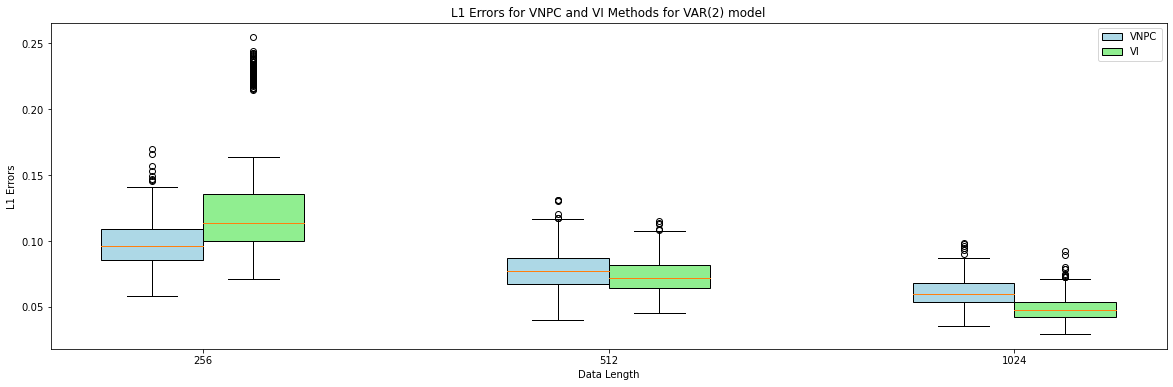
\includegraphics[width=18cm]{L1 Errors for VNPC and VI Methods for VAR(2) model.png}
\end{subfigure}

\begin{subfigure}{\textwidth} % Use \textwidth to fit the width of the text area
  \centering
  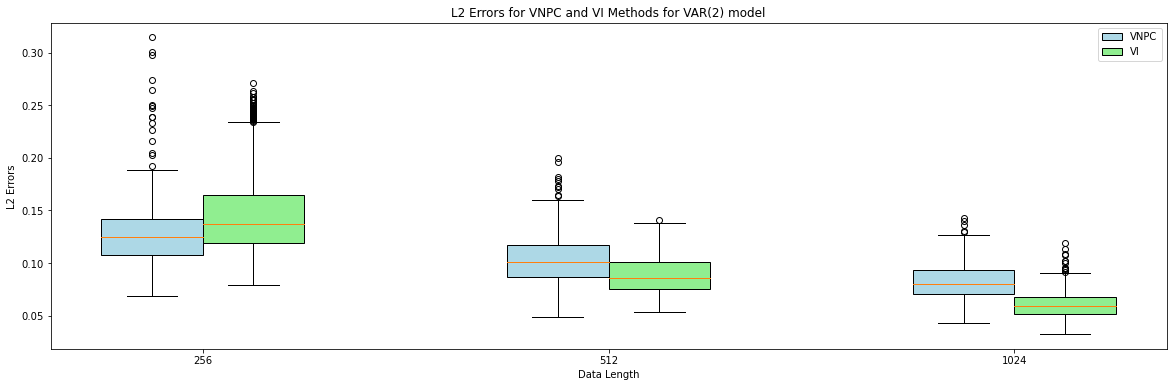
\includegraphics[width=18cm]{L2 Errors for VNPC and VI Methods for VAR(2) model.png}
\end{subfigure}

\caption{The box plots for the distribution of 500 $L_1$ and $L_2$ errors obtained from applying the VNPC and SGVB methods on the VAR(2) model with different sample sizes ($n = 256, 512, 1024$). The blue boxes represent the errors computed by the VNPC method, while the green boxes represent those obtained using variational inference methods, specifically SGVB, as applied in this study.}
\label{l1l2 var2}
\end{figure}

\begin{figure}[H]
\centering
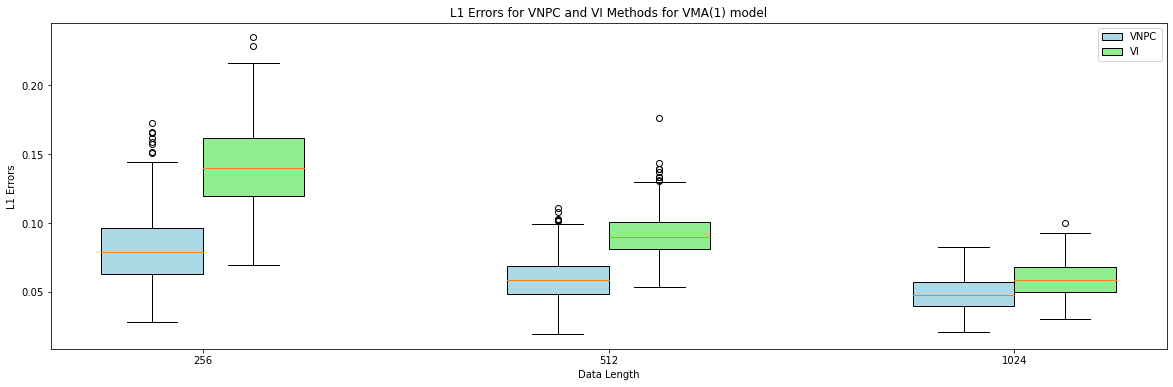
\includegraphics[width=18cm]{L1 Errors for VNPC and VI Methods for VMA(1) model.png}
\end{figure}

\begin{figure}[H]
\begin{subfigure}{\textwidth} % Use \textwidth to fit the width of the text area
  \centering
  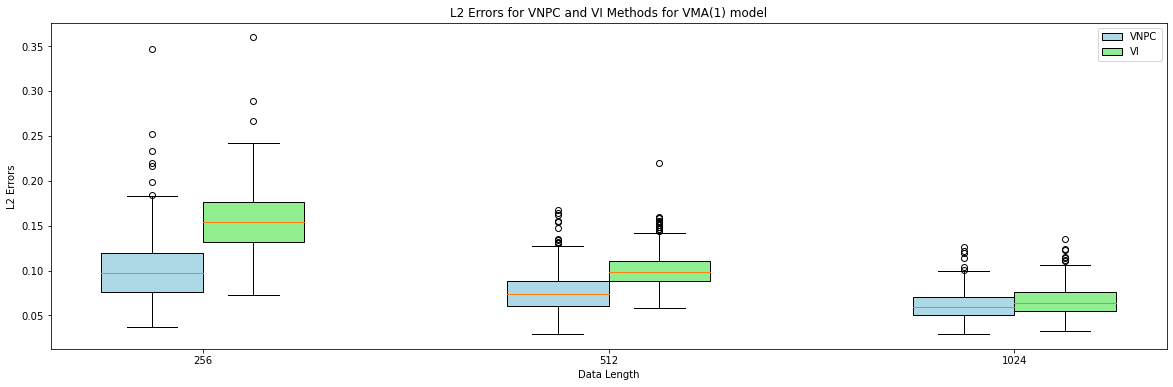
\includegraphics[width=18cm]{L2 Errors for VNPC and VI Methods for VMA(1) model.png}
\end{subfigure}

\caption{The box plots for the distribution of 500 $L_1$ and $L_2$ errors obtained from applying the VNPC and SGVB methods on the VMA(1) model with different sample sizes ($n = 256, 512, 1024$). The blue boxes represent the errors computed by the VNPC method, while the green boxes represent those obtained using variational inference methods, specifically SGVB, as applied in this study.}
\label{plot l1l2 var2}
\end{figure}

The following two tables present the average $L_1$ and $L_2$ errors, as well as the average computation time per realization (in seconds), for the 500 implementations of both models using the VNPC and SGVB methods. \hyperref[table l1l2 var2]{Table 1} corresponds to the VAR(2) model, while the \hyperref[table l1l2 vma1]{Table 2} corresponds to the VMA(1) model:
\begin{table}[h]
\centering
\begin{tabular}{ccccccc}
\hline
\quad & \quad & \quad & {VAR(2) model} & \quad & \quad & \quad\\
\quad & $n=256$ & \quad & $n = 512$ & \quad & $n = 1024$\\
\hline\\
\quad & {VNPC} & {SGVB} & {VNPC} & {SGVB} & {VNPC} & {SGVB}\\
{$L_1$ error} & 0.098 & 0.133 & 0.078 & 0.073 & 0.061 & 0.049\\
{$L_2$ error} & 0.129 & 0.153 & 0.103 & 0.089 & 0.082 & 0.061\\
{Time} & 6066.146 & 23.320 & 10512.16 & 24.079 & 18833.78 & 25.946\\
\hline
\end{tabular}
\caption{Comparison of average $L_1$ and $L_2$ errors, along with the average computation time (in seconds), for 500 realizations using VNPC and SGVB methods across different sample sizes ($n=256$, $512$, and $1024$) for the VAR(2) model.}
\label{table l1l2 var2} 
\end{table}

\begin{table}[h]
\centering
\begin{tabular}{ccccccc}
\hline
\quad & \quad & \quad & {VMA(1) model} & \quad & \quad & \quad\\
\quad & $n=256$ & \quad & $n = 512$ & \quad & $n = 1024$\\
\hline\\
\quad & {VNPC} & {SGVB} & {VNPC} & {SGVB} & {VNPC} & {SGVB}\\
{$L_1$ error} & 0.081 & 0.141 & 0.059 & 0.092 & 0.048 & 0.059\\
{$L_2$ error} & 0.101 & 0.156 & 0.075 & 0.101 & 0.061 & 0.066\\
{Time} & 5432.934 & 27.237 & 8296.563 & 24.070 & 15604.05 & 26.133\\
\hline
\end{tabular}
\caption{Comparison of average $L_1$ and $L_2$ errors, along with the average computation time (in seconds), for 500 realizations using VNPC and SGVB methods across different sample sizes ($n=256$, $512$, and $1024$) for the VMA(1) model.}
\label{table l1l2 vma1} 
\end{table}

When comparing the VNPC method to SGVB, it generally exhibits higher accuracy, except for sample sizes $n=512$ and $n=1024$ in the VAR(2) model, where VNPC's $L_1$ and $L_2$ errors appear to be slightly higher. Additionally, as the sample size increases (from $n=256$ to $n=1024$), the errors obtained by both methods decrease, indicating improved fitting with larger sample sizes. However, the computation time for the VNPC method significantly increases with the sample size, whereas the computation time for the SGVB method remains relatively stable. Therefore, while the VNPC method performs better in reducing errors, it also incurs higher computational costs.

The following plots (Figures \ref{var2 plots} and \ref{vma1 plots}) show the spectral density estimation for one realization of the VAR(2) and VMA(1) models using the VNPC and SGVB methods. For each model, we consider three different sample sizes: $n = 256$, $n = 512$, and $n = 1024$, displayed from top to bottom:
\begin{figure}[H]
\centering
\begin{subfigure}{\textwidth} % Use \textwidth to fit the width of the text area
  \centering
  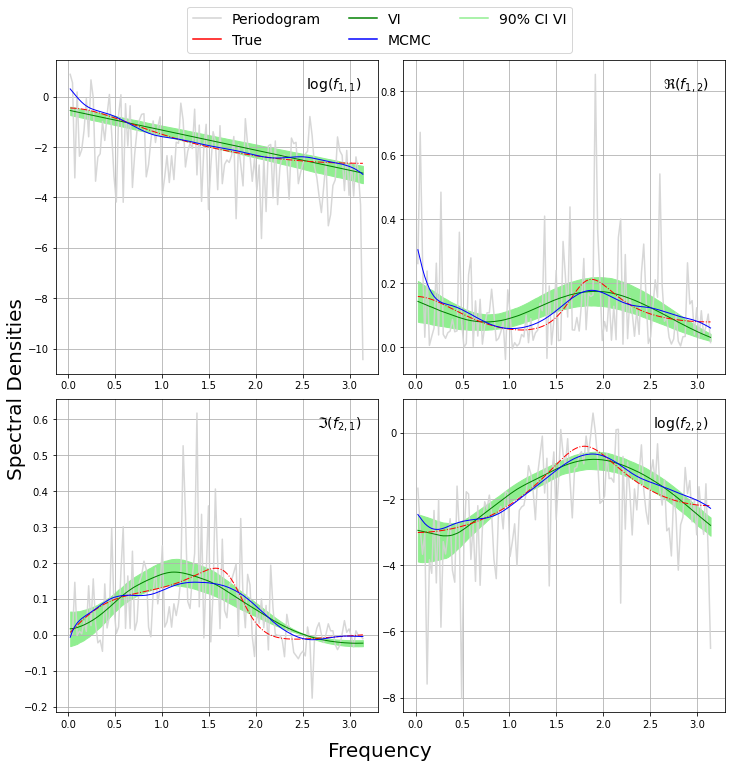
\includegraphics[width=18cm]{VAR(2) with length 256 by variational inference and VNPC.png}
\end{subfigure}

\begin{subfigure}{\textwidth} % Use \textwidth to fit the width of the text area
  \centering
  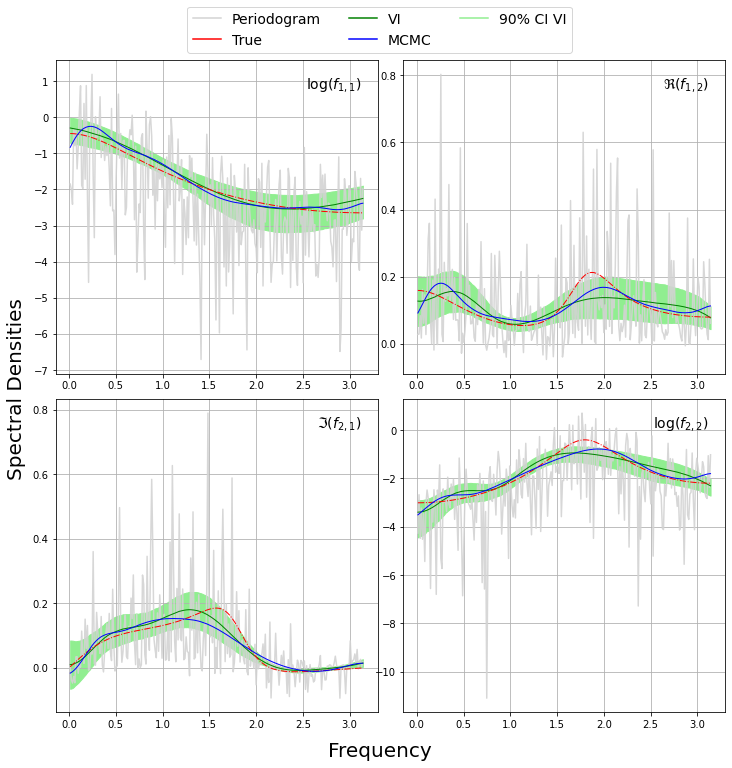
\includegraphics[width=18cm]{VAR(2) with length 512 by variational inference and VNPC.png}
\end{subfigure}

\begin{subfigure}{\textwidth} % Use \textwidth to fit the width of the text area
  \centering
  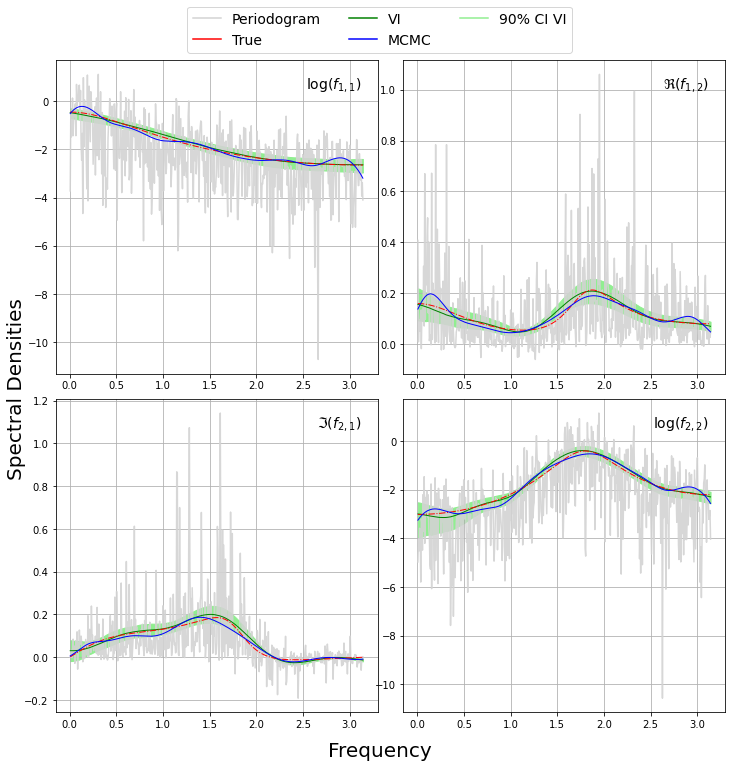
\includegraphics[width=18cm]{VAR(2) with length 1024 by variational inference and VNPC.png}
\end{subfigure}
\caption{Spectral density estimation for one realization of the VAR(2) model with different sample sizes (n = 256, n = 512, and n = 1024) from top to bottom. The legends indicate the following: Red dashed line represents the true spectral density, blue lines depict simulations by SGVB, light pink shadow represents the 95\% confidence interval (CI) of estimation by SGVB, gray lines denote the logarithmic periodogram and empirical cross spectrum, green lines depict simulations by VNPC, and light blue shadow represents the 95\% CI of estimation by VNPC. The plots are presented from left to right, with each column showing the diagonal spectrum, real part, and imaginary part of the cross-spectrum, respectively.}
\label{var2 plots}
\end{figure}

\begin{figure}[H]
\centering
\begin{subfigure}{\textwidth} % Use \textwidth to fit the width of the text area
  \centering
  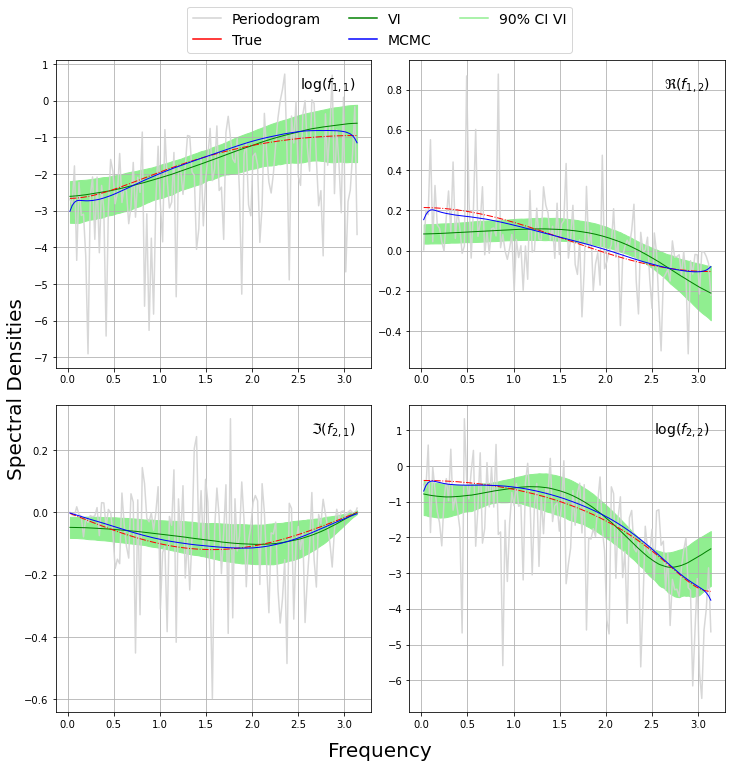
\includegraphics[width=18cm]{VMA(1) with length 256 by variational inference and VNPC.png}
\end{subfigure}

\begin{subfigure}{\textwidth} % Use \textwidth to fit the width of the text area
  \centering
  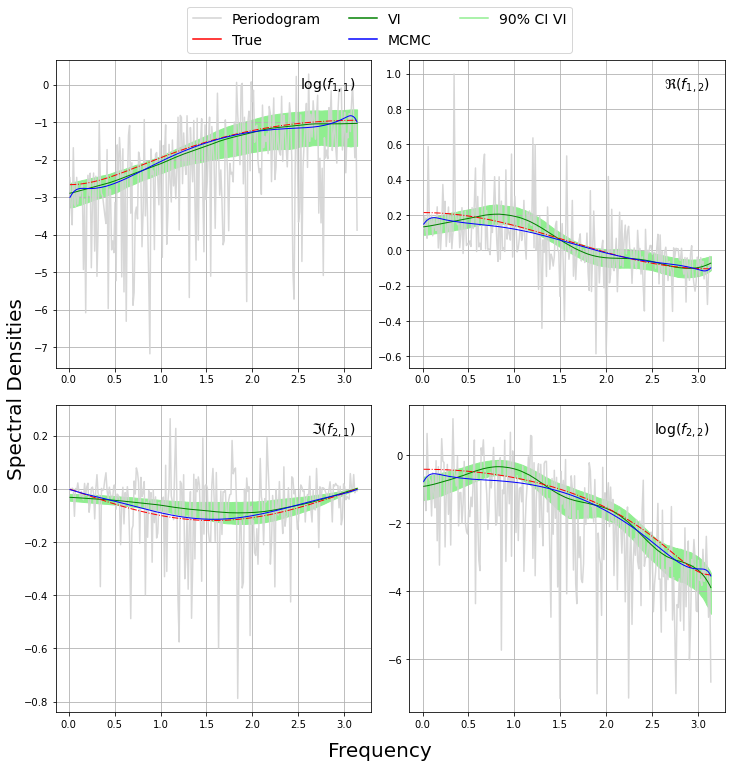
\includegraphics[width=18cm]{VMA(1) with length 512 by variational inference and VNPC.png}
\end{subfigure}

\begin{subfigure}{\textwidth} % Use \textwidth to fit the width of the text area
  \centering
  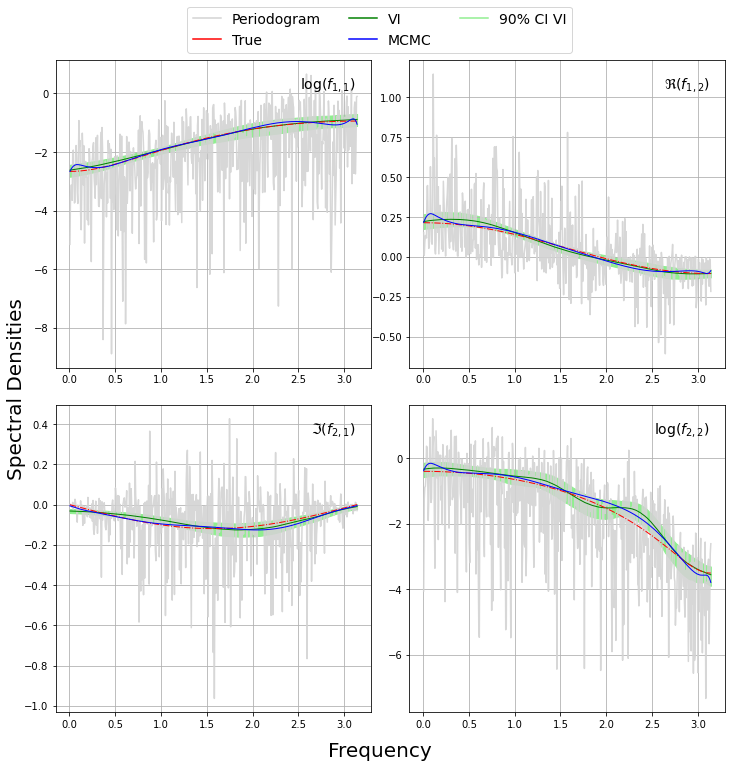
\includegraphics[width=18cm]{VMA(1) with length 1024 by variational inference and VNPC.png}
\end{subfigure}

\caption{Spectral density estimation for one realization of the VAR(2) model with different sample sizes (n = 256, n = 512, and n = 1024) from top to bottom. The legends indicate the following: Red dashed line represents the true spectral density, blue lines depict simulations by SGVB, light pink shadow represents the 95\% confidence interval (CI) of estimation by SGVB, gray lines denote the corresponding periodogram and empirical cross spectrum, green lines depict simulations by VNPC, and light blue shadow represents the 95\% CI of estimation by VNPC. The plots are presented from left to right, with each column showing the diagonal spectrum, real part, and imaginary part of the cross-spectrum, respectively.}
\label{vma1 plots}
\end{figure}

Upon examining Figures \ref{var2 plots} and \ref{vma1 plots}, when the sample size is $n=256$, estimation by SGVB of the VAR(2) model is not particularly accurate, and the estimated spectral density does not coincide with the true one. When the sample size increases, the differences between the estimated spectral density and the true one gradually decreases. However, in the VNPC method, there appears to be some fluctuation in the estimated spectral density, for sample sizes of $n=512$ and $n=1024$. This is also consistent with \hyperref[table l1l2 var2]{Table 1}. SGVB for VMA(1) model are not particularly accurate when the sample size is small, especially noticeable at $n=256$. This discrepancy between SGVB simulations and the true spectral density is pronounced. In contrast, VNPC maintains a closer approximation to the true values, even with smaller sample sizes. As the sample size increases, the simulations of both methods gradually converge towards the true spectral density.

\subsection{Application}
The Southern Oscillation Index (SOI) and the associated recruitment series (REC) are two simultaneously recorded time series, which are believed to be related to the El Niño Southern Oscillation (ENSO) phenomenon. The SOI is a standardized index based on the sea level pressure differences between Tahiti and Darwin, Australia. The recruitment series, on the other hand, represents the number of newly spawned fish, which is thought to be influenced by the water temperature. As ENSO is known to affect the sea surface temperature and air pressure across the equatorial Pacific Ocean, a cross-dependence between the SOI and the REC series can be expected. For this analysis, we use the SOI and REC datasets available in the R package "astsa". Both series include 453 monthly values from 1950 to 1987. The recruitment series is re-scaled to the interval [0, 100], and both series are standardized to have zero mean and unit variance. Our goal is to estimate the spectral densities of the individual series and the cross-spectral density between them, in order to investigate their frequency-domain properties and correlation.

The SGVB is used to simulate the spectral densities, the number of basis functions is set to 50, and the step
sizes are set to be 0.05 for both phases.
\begin{figure}[h]
\begin{minipage}[b]{0.45\linewidth}
\centering
\includegraphics[width=200pt]{soi 50 0.05.png}
\end{minipage}
\begin{minipage}[b]{0.45\linewidth}
\centering
\includegraphics[width=200pt]{rec 5 0 0.05.png}
\end{minipage}

\begin{minipage}[b]{0.45\linewidth}
\centering
\includegraphics[width=200pt]{ref12 5 0 0.05.png}
\end{minipage}
\begin{minipage}[b]{0.45\linewidth}
\centering
\includegraphics[width=200pt]{imf12 50 0.05.png}
\end{minipage}
\caption{Logarithmic spectral estimates for the SOI and REC series (top row), and the real and imaginary parts of the cross-spectrum estimation (bottom row). Legend: Blue lines indicate simulated spectral densities by SGVB; pink shaded areas represent 95\% confidence intervals; gray lines depict corresponding periodograms and empirical cross spectrum.}
\label{soi}
\end{figure}

The squared coherence is used to investigate the correlation between two series. If the value of squared coherence $\rho_{ij}^2(\nu_k)$ is closer to 1, this means the two series have a strong association. If it is closer to 0, this indicates the association is very weak between the two series. Recall that the squared coherence $\rho_{ij}^2(\nu_k)$ between two series for frequency $\nu_k$ is defined as:
\begin{align}
\rho_{ij}^2(\nu_k) = \frac{|\bm{f}_{ij}(\nu_k)|^2}{\bm{f}_{ii}(\nu)\bm{f}_{jj}(\nu_k)}
\end{align}
where $\bm{f}_{ij}(\nu_k)$ for $i,j = 1,2,...,p$ and $i\neq j$ represents the cross-spectral density between series $i$ and $j$ at frequency $\nu_k$, while $\bm{f}_{ii}(\nu_k)$ and $\bm{f}_{jj}(\nu_k)$ represent the spectral densities of series $i$ and $j$, respectively, at frequency $\nu_k$.

The estimated squared coherency between SOI and REC obtained through SGVB is depicted as:
\begin{figure}[H]
\centering
\includegraphics[width=11cm]{coherency 50 0.05.png}
\caption{Estimated squared coherence between SOI and REC by SGVB. In the legend, the blue line represents the simulation, while the pink shadow denotes the 95\% Confidence Interval (CI).}
\label{coherency 50 0.05}
\end{figure}

From Figure \ref{soi}, the periodograms of both SOI and REC series show a prominent peak at the frequency $\nu \approx 0.52$. This frequency corresponds to a period of 12 months since $\nu = \frac{2\pi}{12}\approx 0.52$, indicating a strong annual periodicity in both series. From Figure \ref{coherency 50 0.05}, a clear peak can be observed at $\nu\approx 0.52$. This suggests that the SOI and REC series are strongly correlated at the annual frequency. Additional peaks at higher frequencies indicate significant correlations between the two series at other periodicities as well.







\section{So What's New?}
\label{sec:whatsnew}
\subsection{Wind speed profiles}
The SGVB method is employed to estimate the spectral density of wind speed data collected from six different airports in California. The data spans from 01-06-2019 12:00 am to 31-08-2019 11:59 pm and includes observations from the following locations: EDU (Davis), SAC and SMF (Sacramento), MRY (Monterey), SNS (Salinas), and WVI (Watsonville). Each data point represents the median wind speed for every two hours at each location. The dataset comprises a 6-dimensional multivariate time series with a total length of 1104. Prior to analysis, the data is standardized and detrended. Notably, SMF, SAC, and EDU form a distinct group due to their proximity, while the remaining three locations are also clustered together within their own distinct area, they are situated farther apart from the are that containing SMF, SAC, and EDU.
\begin{figure}[H]
\centering
\includegraphics[width=5cm]{6 locations.jpg}
\caption{Locations for the six places.}
\end{figure}

The squared coherence between pairs of different locations is analyzed using SGVB. As reported by \hyperref[hu2023]{Hu and Prado (2023)}, nonzero squared coherence values only manifest locally. Specifically, a noticeable association is observed between two locations if they are close to each other spatially. Conversely, when the pair of locations are distant from each other—such as one location being from EDU, SAC, or SMF, and the other from MRY, SNS, or WVI, then the squared coherence is zero. In their research, the number of basis functions is set to 30, and the step sizes are set to be 0.001 and 0.05, respectively for each phase

To explore the potential correlation between wind speed datasets for different pairs of places, the empirical squared coherence is computed using the Python function signal.coherence. This function divides each signal into overlapping segments, each of which is windowed (commonly with a Hanning window) and then subjected to a Fast Fourier Transform (FFT) to produce a periodogram for each segment. The Power Spectral Density (PSD) for each signal is then estimated by averaging the periodograms of the segments, while the Cross Spectral Density (CSD) between the signals is obtained in a similar manner. Thus, the empirical squared coherence is calculated by dividing the magnitude-squared of the CSD by the product of the PSDs for the two signals. In this study, the length of each segment is set to be 100, with each segment overlapping by 50 data points with the preceding segment.

The following two plots (Figures \ref{wind speed psd} and \ref{wind speed coh}) depict estimated logarithmic spectral densities for six different locations, as well as estimated squared coherences by SGVB and empirical squared coherences between pairs of different locations. The step sizes for both phases are set to 0.1, and the number of basis functions is set to 30:
\begin{figure}[H]
\centering
\includegraphics[width=14cm]{psd for wind speed.png}
\caption{Logarithmic spectral density estimates for wind speed data at six locations using SGVB. Legend: Blue lines indicate simulated spectral densities by SGVB; pink shaded areas represent 95\% confidence intervals; gray lines depict corresponding periodograms.}
\label{wind speed psd}
\end{figure}

\begin{figure}[H]
\centering
\includegraphics[width=14cm]{new sq coh for wind speed.png}
\caption{Estimated squared coherence for wind speed data between pairs of different locations. Legend: Blue lines represent simulated squared coherence by SGVB; Green lines represent empirical squared coherences; pink shaded areas indicate 95\% confidence intervals.}
\label{wind speed coh}
\end{figure}

From Figure \ref{wind speed psd}, it is evident that for every estimated spectral density, the first prominent peak appears at $\nu \approx 0.083$. This suggests a strong daily periodicity for each location, given that there are 12 observations per day ($\nu = \frac{1}{12} \approx 0.083$). Moreover, the spectral density estimations near $\nu = 0.083$ for coastal areas (WVI, SNS, MRY) exhibit slightly higher amplitudes compared to those for inland areas. These findings are consistent with those reported by \hyperref[hu2023]{Hu and Prado (2023)}.

From Figure \ref{wind speed coh}, the squared coherence for every pair of locations is very clear, the most obvious peak appear for every pair of locations is at $\nu=0.083$, this means the information of the wind speed is strongly correlated across all locations at this frequency. The results are consistent with the one from  \hyperref[liu 2023]{Liu et al. (2023)}. Nearly all empirical squared coherences between different pairs of locations fall within the 95\% confidence intervals of their corresponding estimated squared coherences by SGVB. This indicates that the step size for phase 1 has a significant impact on estimated spectral density and squared coherence. For SGVB, a reasonable larger step size appears to capture more characteristics of the time series in the spectral density and coherence. However, the underlying reasons and principles behind this phenomenon are still under investigation.






\subsection{Einstein Telescope}
The Einstein Telescope is a proposed next-generation gravitational wave detector. It is designed to have a triangular configuration, consisting of three Michelson interferometers, called X, Y, and Z. Each side of the triangle will be 10 kilometers long, and the angle between the adjacent sides will be 60 degrees. To reduce the effects of seismic noise, ET will be built a few hundred meters underground. The test mass is a stable and highly reflective surface, with a weight of approximately 120 kg each, and to reduce thermal noise, the test mass will be kept at 20 Kelvin. ET will use 500 watts high-power lasers, combined with the use of squeezed light to reduce the quantum noise. ET will optimize both low and high frequency sensitivity, which is expected to be much higher than current advanced second-generation detectors such as advanced LIGO and advanced Virgo.

To simulate the presence of non-identical correlated noise on X, Y and Z channels, \hyperref[janssens2022]{Janssens et al. (2022)} artificially injected some Gaussian peak noise in the frequency domain. Gaussian noise was injected on the X channel at 10 Hz and 50 Hz. For Y channel, the Gaussian noise was injected at 10 Hz and 90 Hz. For Z channel, the Gaussian noise was injected at 50 Hz and 90 Hz. Then, there is a correlated Gaussian noise peak between each pair of channels.

In this study, the SGVB method is utilized to estimate the spectral densities for the simulated data of three channels, and construct the coherences for every pair of channels to obtain the correlation between then in the certain frequencies. The dataset can be considered as a  three dimensional Gaussian stationary multivariate time series with length 4194304.

To handle such a large data set, in this study, the whole dataset is evenly divided into 400 segments, with the remaining segment of length 304 being discarded. Each segment can be regarded as a three dimensional multivariate time series with a length of 10485. The Fourier-transformed version of each segment serves as input data for a Whittle likelihood. Every Whittle likelihood with corresponding input segment has the same basis function expressions for spectral density matrix. Since the Fourier transform is an even function, the number of frequency points for each segment is now 5242. Consequently, the product of 400 Whittle likelihoods from corresponding segments forms a new Whittle likelihood representing almost the entire dataset. The expression of the new Whittle likelihood is given below:
\begin{align}
p^{n}_W(\mathbf{y}(\nu_1), \ldots, \mathbf{y}(\nu_N)| \bm{f}) \propto 
\prod_{j=1}^{J} \left(\prod_{l=1}^{L} \det(\bm{f}(\nu_l))^{-1} \exp\left(-\mathbf{y}^{(j)}(\nu_l)^* \bm{f}(\nu_l)^{-1} \mathbf{y}^{(j)}(\nu_l)\right)\right)
\end{align}
where $j = 1, \dots, J$ means the number of segments, in this case $J = 400$, $l = 1, \dots, L$ means the length of each input segment, in this case $L = 5242$.

In this case, the hyperparameter $b$ in the regularized horseshoe prior is modified to $b=M$, where $M$ is the number of basis functions. This choice allows the model to utilize a larger number of basis functions (up to 750). The increased flexibility enables the model to capture more complex patterns in the data. The step sizes are set to be 0.01 and 0.05, respectively for each phase.

The following plots show the estimated spectral densities for three channels, as well as the estimated squared coherences for different pairs of channels by SGVB:
\begin{figure}[H]
\centering
\begin{subfigure}{\textwidth} % Use \textwidth to fit the width of the text area
  \centering
  \includegraphics[width=12cm]{power spectrum for x channel.png}
\end{subfigure}

\begin{subfigure}{\textwidth} % Use \textwidth to fit the width of the text area
  \centering
  \includegraphics[width=12cm]{power spectrum for y channel.png}
\end{subfigure}

\begin{subfigure}{\textwidth} % Use \textwidth to fit the width of the text area
  \centering
  \includegraphics[width=12cm]{power spectrum for z channel.png}
\end{subfigure}

\caption{The estimated spectral densities for three channels on a logarithmic scale for the first 100 Hz. The green lines represent the estimated spectral densities by SGVB, the grey lines represent the corresponding periodograms.}
\label{psd channels}
\end{figure}

\begin{figure}[H]
\centering
\begin{subfigure}{\textwidth} % Use \textwidth to fit the width of the text area
  \centering
  \includegraphics[width=15cm]{squared coherence for xy channel.png}
\end{subfigure}

\begin{subfigure}{\textwidth} % Use \textwidth to fit the width of the text area
  \centering
  \includegraphics[width=15cm]{squared coherence for xz channel.png}
\end{subfigure}

\begin{subfigure}{\textwidth} % Use \textwidth to fit the width of the text area
  \centering
  \includegraphics[width=15cm]{squared coherence for yz channel.png}
\end{subfigure}
\caption{The estimated squared coherences between pairs of channels. The green lines represent the estimated squared coherences by SGVB, pink shaded areas indicate 95\% confidence intervals.}
\label{coh channels}
\end{figure}

From Figure \ref{psd channels}, it is evident that in the X channel, prominent peaks are observed at 10 Hz and 50 Hz. Similarly, for the Y channel, peaks are observed at 10 Hz and 90 Hz, while for the Z channel, peaks are observed at 50 Hz and 90 Hz. From Figure \ref{coh channels}, it is evident that there is significant coherence between channels X and Y at 10 Hz, between channels X and Z at 50 Hz, and between channels Y and Z at 90 Hz. The results are consistent with the one from \hyperref[janssens2022]{Janssens et al. (2022)}. 





\section{Goals}
\begin{enumerate}
    \item Explore hyperparameter optimization in order to set the optimal step size, explore the effect of any other hyperparameter choices of the VB algorithm, re-run a simulation study, apply this approach to estimating the correlated noise from gravitational waves observed by the three channels of the Einstein Telescope, and then write and submit a paper to an astrophysics and/or applied statistics journal. 
    
    01/05/2024 - 30/10/2024
    
    \item Explore coarsened (Gamma) likelihood instead of Whittle likelihood in combination with VB.

    01/11/2024 - 28/02/2025

    \item Using  simulated correlated noise of three ET channels (or LISA channels) , inject a gravitational wave signal to the noise and estimate the parameters of signal and noise spectral density simultaneously using a Gibbs sampler, and then write and submit a paper to Physical Review D (PRD).
    
    01/03/2024 - 30/9/2025

    \item Time permitting: explore subsampling approach for speeding up spectral density estimation when dealing with huge time series.

    01/10/2025 - 31/01/2026

    \item Complete the final thesis.

    01/02/2026 - 30/05/2026
\end{enumerate}

\section{Deliverables and Program Schedule}
All AFA provisional goals:
\begin{enumerate}


\item
\textit{Approval of the full thesis proposal by the Confirmation Review Committee}: In progress.


\item
\textit{A substantial piece of written work, completed to the satisfaction of the supervisors and the Confirmation Review
Committee}: Submitted.


\item
\textit{Discussion with the Confirmation Review Committee of the full thesis proposal, written work, research plan and other
thesis-related work, to the satisfaction of the Committee}:
In progress.

\item
\textit{An oral presentation on their doctoral work to the satisfaction of the Confirmation Review Committee}:
In progress.

\item
\textit{Ethics approval(s)/permissions obtained for the research
(if required)}:
Not necessary.

\item
\textit{Completion of the central University induction, within the first 2 months of candidature}:
Completed.


\item
\textit{Diagnostic English Language Needs Assessment (DELNA) online screening, within the first 2 months of candidature and
i) completion of full diagnostic test where prescribed, and
ii) completion, with at least a B result, of any language course prescribed by the DELNA Language Adviser, and
iii) participation in any language enrichment prescribed by the DELNA Language Adviser}:
Completed.


\item
\textit{Successful completion of the University’s academic integrity training}:
Completed.



\item
\textit{A training and development needs analysis, within the first 6 months of candidature}:
Completed.


\item
\textit{Completion of a health and safety risk assessment and training for any laboratory/studio/field and related work, if
required for the initial period of candidature.}:
Not necessary.



\item
\textit{Enrol into STATS 731 and 782 and achieve a grade of B+ or higher}:
B- for STATS 782, A- for STATS 731.

\item
\textit{Produce a literature review on Bayesian spectral density estimation and variational Bayes methods, to the satisfaction of
the primary supervisor}:
Submitted.

\item
\textit{Attendance at one of the Faculty of Science Doctoral Induction Workshops}:
Completed.

\item
\textit{Attend at least 10 relevant research presentations per annum (student needs to verify participation by filling out and
handing in the departmental attendance form for each presentation to the Statistics Department office).}:
Completed.

\item
\textit{Participate in the Department of Statistics PhD Talks Day and/or give a departmental seminar, to the satisfaction of the
main supervisor}:
In progress.

\item
\textit{Maintain a personal profile page (www.directory.auckland.ac.nz), providing information on scholarly activities and
objectives, to the satisfaction of the main supervisor and a Department of Statistics PhD Officer}:
In progress.


\end{enumerate}









\begin{table}[hh]
\caption{
Departmental seminars I have attended (top part of the table).
Talks from another UoA department are in the middle tier.
Conferences and workshops are in the bottom tier,
e.g., 2019-05-29 event was an all-day workshop.
\textbf{Note}:
I filled in the required document and submitted it
within the required time period after
each seminar I attended.
}
\centering
\ ~~~~ \\
\label{tab:seminars}
\begin{tabular}{|c|l|l|}
\hline
Date & Speaker & Title \\
\hline
2022-11-18 & Ellen Powell &
Characterising the Gaussian free field \\
%
2023-11-18 & Juan Carlos Pardo &
\parbox{10cm}{Growth fragmentation embedded in Brownian excursions from hyperplanes} \\
%

2022-11-22 & Richard Barker &
Bayesian Foundation of Multimodel Inference \\
%
2023-02-28 & Markus Neuhaeuser &
\parbox{10cm}{The propensity score for the analysis of observational studies} \\
%
2023-02-10 & Rob Gould &
K-12 Data Science or stats? \\
%
2023-07-12 & Cristian Felipe Jimenez Varon &
\parbox{10cm}{Forecasting high-dimensional functional time series: Application to sub-national age-specific mortality} \\
%
2023-09-15 & Roberto Armellin &
High-order methods in astrodynamics \\
%
2023-08-22 & Sean Carroll &
Euler characteristics of groups \\
%
2023-08-23 & Mauren Porciuncula &
\parbox{10cm}{Teaching knowledge, playfulness, student protagonist, social justice, interdisciplinarity: some results of Brazilian research in statistical education} \\
%
2023-08-29 & Vincent Geiger &
\parbox{10cm}{The role of Critical Mathematical Thinking in responding to disruptive phenomena} \\
%

\hline
\end{tabular}
\end{table}




\newpage
\textbf{References}

\begin{enumerate}
\item \label{caprini2018} Caprini, C., \& Figueroa, D. G. (2018). Cosmological backgrounds of gravitational waves. \textit{arXiv preprint}, arXiv:1801.04268.

\item \label{BD1991} Brockwell, P. J., \& Davis, R. A. (1991). \emph{Time series: Theory and methods}. Springer, New York, 2nd edition.

\item \label{Samaniego (2010)} Samaniego, F. J. (2010). \emph{A comparison of the Bayesian and frequentist approaches to estimation}. New York: Springer.

\item \label{Kreiss2011} Kreiss, J.-P., Paparoditis, E., \& Politis, D. N. (2011). On the range of validity of the autoregressive sieve bootstrap. \emph{Annals of Statistics, 39}(4), 2103-2130. \url{https://doi.org/10.1214/11-AOS900}.

\item \label{Krampe2019} Krampe, J., Kreiss, J.-P., \& Paparoditis, E. (2019). Bootstrap based inference for sparse high-dimensional time series models. \emph{arXiv preprint}, arXiv:1806.11083v3.

\item \label{han2013} Han, F., Lu, H., \& Liu, H. (2013). A direct estimation of high dimensional stationary vector autoregressions. \textit{Journal of Machine Learning Research}, 16, 3115-3150.

\item \label{kastner2020} Kastner, G., \& Huber, F. (2020). Sparse Bayesian vector autoregressions in huge dimensions. \emph{Journal of Forecasting}, 39, 1142–1165. \url{https://doi.org/10.1002/for.2680}.

\item \label{ni2005} Ni, S., \& Sun, D. (2005). Bayesian Estimates for Vector Autoregressive Models. \emph{Journal of Business \& Economic Statistics}, \emph{23}(1), 105–117. \url{http://www.jstor.org/stable/27638798}.

\item \label{chan2020} Chan, J. C. C. (2020). Large Bayesian Vector Autoregressions. In P. Fuleky (Ed.), \emph{Macroeconomic Forecasting in the Era of Big Data} (Advanced Studies in Theoretical and Applied Econometrics, Vol. 52). Springer. \url{https://doi.org/10.1007/978-3-030-31150-6_4}.

\item \label{Holand 2017} Holan, S. H., McElroy, T. S., \& Wu, G. (2017). The cepstral model for multivariate time series: The vector exponential model. \emph{Statistica Sinica, 27}(1), 23–42. \url{http://www.jstor.org/stable/44114360}.

\item \label{Villani (2022)} Villani, M., Quiroz, M., Kohn, R., \& Salomone, R. (2022). Spectral Subsampling MCMC for Stationary Multivariate Time Series with Applications to Vector ARTFIMA Processes. \emph{Econometrics and Statistics}, ISSN 2452-3062. \url{https://doi.org/10.1016/j.ecosta.2022.10.001}.

\item \label{Jentsch2010} Jentsch, C., \& Kreiss, J.-P. (2010). The multiple hybrid bootstrap - resampling multivariate linear processes. \emph{Journal of Multivariate Analysis}, \emph{101}(10), 2320–2345. \url{https://doi.org/10.1016/j.jmva.2010.06.005}.

\item \label{Jentsch2015} Jentsch, C., \& Politis, D. N. (2015). Covariance matrix estimation and linear process bootstrap for multivariate time series of possible increasing dimension. \emph{Annals of Statistics, 43}(3), 1117–1140. \url{https://doi.org/10.1214/14-AOS1301}.

\item \label{Meyer2020} Meyer, M., Paparoditis, E., \& Kreiss, J.-P. (2020). Extending the validity of frequency domain bootstrap methods to general stationary processes. \emph{The Annals of Statistics, 48}, 2402–2427.

\item \label{meyer2023} Meyer, M., \& Paparoditis, E. (2023). A frequency domain bootstrap for general multivariate stationary processes. \emph{Bernoulli, 29}(3), 2367–2391. \url{https://doi.org/10.3150/22-BEJ1545}.

\item \label{whittle} Whittle, P. (1957). Curve and periodogram smoothing. \emph{Journal of the Royal Statistical Society. Series B (Methodological)}, \emph{19}(1), 38–63. \url{https://doi.org/10.1111/j.2517-6161.1957.tb00242.x}.

\item \label{rosen-stoffer-2007} Rosen, O., Stoffer, D.S. (2007). Automatic estimation of multivariate spectra via smoothing splines. \emph{Biometrika}, \textit{94}(2), 335–345. DOI: 10.1093/biomet/asm022.

\item \label{Krafty 2013} Krafty, R. T., \& Collinge, W. O. (2013). Penalized multivariate Whittle likelihood for power spectrum estimation. \emph{Biometrika}, \textit{100}(2), 447–458. \url{https://doi.org/10.1093/biomet/ast012}.

\item \label{Holbrook 2018} Holbrook, A., Lan, S., Vandenberg-Rodes, A., \& Shahbaba, B. (2018). Geodesic Lagrangian Monte Carlo over the space of positive definite matrices: with application to Bayesian spectral density estimation. \emph{Journal of Statistical Computation and Simulation}, \textit{88}(5), 982-1002. \url{https://doi.org/10.1080/00949655.2017.1416470}.

\item \label{Meier 2018} Meier, A., Kirch, C., \& Meyer, R. (2020). Bayesian nonparametric analysis of multivariate time series: A matrix Gamma Process approach. \emph{Journal of Multivariate Analysis}, \textit{175}, 104560. \url{https://doi.org/10.1016/j.jmva.2019.104560}.

\item \label{liu 2023} Liu, Y., Kirch, C., Lee, J. E., \& Meyer, R. (2023). A nonparametrically corrected likelihood for Bayesian spectral analysis of multivariate time series. \emph{arXiv preprint}, arXiv:2306.04966.

\item \label{hu2023} Hu, Z., \& Prado, R. (2023). Fast Bayesian inference on spectral analysis of multivariate stationary time series. \textit{Computational Statistics \& Data Analysis}, \emph{178}, Article 107596. \url{https://doi.org/10.1016/j.csda.2022.107596}.

\item \label{gg2023} Granados-Garcia, G., Prado, R., \& Ombao, H. (2023). Bayesian nonparametric multivariate mixture of autoregressive processes: With application to brain signals. \emph{arXiv preprint}, arXiv:2305.08790.

\item \label{2004a} Choudhuri, N., Ghosal, S., \& Roy, A. (2004). Bayesian Estimation of the Spectral Density of a Time Series. \emph{Journal of the American Statistical Association}, \textit{99}, 1050-1059. \url{https://doi.org/10.1198/016214504000000557}.

\item \label{kirch2019} Kirch, C., Edwards, M. C., Meier, A., \& Meyer, R. (2019). Beyond Whittle: Nonparametric Correction of a Parametric Likelihood with a Focus on Bayesian Time Series Analysis. \emph{Bayesian Analysis}, \textit{14}(4), 1037-1073. \url{https://doi.org/10.1214/18-BA1126}.

\item \label{edwards2019} Edwards, M. C., Meyer, R., \& Christensen, N. (2019). Bayesian nonparametric spectral density estimation using B-spline priors. \emph{Statistical Computing}, \textit{29}(1), 67–78. \url{https://doi.org/10.1007/s11222-017-9796-9}.

\item \label{russel2021} Maturana-Russel, P., \& Meyer, R. (2021). Bayesian spectral density estimation using P-splines with quantile-based knot placement. \emph{Computational Statistics}, \textit{36}(3), 2055–2077. \url{https://doi.org/10.1007/s00180-021-01066-7}.

\item \label{blei2017} David M. Blei, Alp Kucukelbir \& Jon D. McAuliffe (2017). Variational Inference: A Review for Statisticians, \emph{Journal of the American Statistical Association}, \emph{112}(518), 859-877. DOI: \href{https://doi.org/10.1080/01621459.2017.1285773}{10.1080/01621459.2017.1285773}.

\item \label{wang2019} Wang, Y., \& Blei, D. M. (2019). Frequentist consistency of variational Bayes. \emph{Journal of the American Statistical Association}, \emph{114}(527), 1147--1161. \url{https://doi.org/10.1080/01621459.2018.1473776}.

\item \label{bishop2006} Bishop, C. M. (2006). \textit{Pattern recognition and machine learning}. Springer New York.

\item \label{blei2006} Blei, D. M., \& Jordan, M. I. (2006). Variational inference for Dirichlet process mixtures. \emph{Bayesian Analysis}, \emph{1}(1), 121--143. \url{https://doi.org/10.1214/06-BA104}.

\item \label{giordano2015} Giordano, R. J., Broderick, T., \& Jordan, M. I. (2015). Linear response methods for accurate covariance estimates from mean field variational Bayes. \emph{Advances in Neural Information Processing Systems}, \emph{28}.

\item \label{han2019} Han, W., \& Yang, Y. (2019). Statistical inference in mean-field variational Bayes. \emph{arXiv preprint}, arXiv:1911.01525.

\item \label{kingma2013} Kingma, D. P., \& Welling, M. (2014). Auto-Encoding Variational Bayes. \emph{arXiv preprint arXiv:1312.6114.} \url{https://doi.org/10.48550/arXiv.1312.6114}.

\item \label{xu2019} Xu, M., Quiroz, M., Kohn, R., \& Sisson, S. A. (2019). Variance reduction properties of the reparameterization trick. \textit{arXiv preprint}, arXiv:1809.10330v3.

\item \label{miller2016} Miller, A. C., Foti, N., \& Adams, R. P. (2016). Variational Boosting: Iteratively Refining Posterior Approximations. \textit{arXiv preprint}, arXiv:1611.06585v2.

\item \label{domke2019} Domke, J. (2019). Provable Gradient Variance Guarantees for Black-Box Variational Inference. \textit{arXiv preprint}, arXiv:1906.0824v2.

\item \label{Kucukelbir2016} Kucukelbir, A., Tran, D., Ranganath, R., Gelman, A., \& Blei, D. M. (2017). Automatic differentiation variational inference. \textit{Journal of Machine Learning Research}.

\item \label{rezende2015} Rezende, D., \& Mohamed, S. (2015). Variational inference with normalizing flows. In \emph{Proceedings of the 32nd International Conference on Machine Learning} (\emph{Proceedings of Machine Learning Research}, Vol. 37, pp. 1530--1538). Retrieved from \url{https://proceedings.mlr.press/v37/rezende15.html}.

\item \label{tan2018} Tan, L. S., \& Nott, D. J. (2018). Gaussian variational approximation with sparse precision matrices. \textit{Statistics and Computing, 28}(2), 259–275. \url{https://doi.org/10.1007/s11222-017-9729-7}.

\item \label{papa2021} Papamakarios, G., Nalisnick, E., Rezende, D. J., Mohamed, S., \& Lakshminarayanan, B. (2021). Normalizing flows for probabilistic modeling and inference. \emph{Journal of Machine Learning Research}, \emph{22}(1), Article 57.

\item \label{archer2016} Archer, E., Park, I. M., Buesing, L., Cunningham, J., \& Paninski, L. (2016). Black box variational inference for state space models. \textit{arXiv preprint}, arXiv:1511.07367.

\item \label{ong2018} Ong, V. M.-H., Nott, D. J., \& Smith, M. S. (2018). Gaussian variational approximation with a factor covariance structure. \textit{Journal of Computational and Graphical Statistics, 27}(3), 465–478. \url{https://doi.org/10.1080/10618600.2017.1390472}.

\item \label{quiroz2020} Quiroz, M., Nott, D.J., \& Kohn, R. (2020). Gaussian variational approximation for high-dimensional state space models. \textit{arXiv preprint}, arXiv:1801.07873.

\item \label{mnih2014} Mnih, A., \& Gregor, K. (2014). Neural variational inference and learning in belief networks. In \emph{Proceedings of the International Conference on Machine Learning} (pp. 1791--1799). PMLR.

\item \label{hoff2013} Hoffman, M. D., Blei, D. M., Wang, C., \& Paisley, J. (2013). Stochastic variational inference. \emph{Journal of Machine Learning Research}.

\item \label{paisley2012} Paisley, J., Blei, D., \& Jordan, M. (2012). Variational Bayesian inference with stochastic search. \textit{arXiv preprint}, arXiv:1206.6430.

\item \label{ranganath2014} Ranganath, R., Gerrish, S., \& Blei, D. (2014, April). Black box variational inference. In \textit{Artificial intelligence and statistics} (pp. 814-822). PMLR.

\item \label{mandt2017} Mandt, S., Hoffman, M. D., \& Blei, D. M. (2017). Stochastic Gradient Descent as Approximate Bayesian Inference. \textit{arXiv preprint}, arXiv:1704.04289v2.

\item \label{lim2021} Lim, K.-L., \& Jiang, X. (2021). Variational posterior approximation using stochastic gradient ascent with adaptive stepsize. \textit{Pattern Recognition}, \textit{112}, 107783. \url{https://doi.org/10.1016/j.patcog.2020.107783}.

\item \label{gershman2012} Gershman, S., Hoffman, M., \& Blei, D. (2012). Nonparametric variational inference. \textit{arXiv preprint}, arXiv:1206.4665.

\item \label{pii2017} Carvalho, C. M., Polson, N. G., \& Scott, J. G. (2017). Sparsity information and regularization in the horseshoe and other shrinkage priors. \textit{Electronic Journal of Statistics, 11}, 5018–5051. \url{https://doi.org/10.1214/17-EJS1337SI}.

\item \label{janssens2022} Janssens, K., Boileau, G., Bizouard, M.-A., Christensen, N., Regimbau, T., \& van Remortel, N. (2022). Formalism for power spectral density estimation for non-identical and correlated noise using the null channel in Einstein Telescope. \textit{arXiv preprint}, arXiv:2205.00416.

\end{enumerate}

\end{document}